\documentclass[1p]{elsarticle_modified}
%\bibliographystyle{elsarticle-num}

%\usepackage[colorlinks]{hyperref}
%\usepackage{abbrmath_seonhwa} %\Abb, \Ascr, \Acal ,\Abf, \Afrak
\usepackage{amsfonts}
\usepackage{amssymb}
\usepackage{amsmath}
\usepackage{amsthm}
\usepackage{scalefnt}
\usepackage{amsbsy}
\usepackage{kotex}
\usepackage{caption}
\usepackage{subfig}
\usepackage{color}
\usepackage{graphicx}
\usepackage{xcolor} %% white, black, red, green, blue, cyan, magenta, yellow
\usepackage{float}
\usepackage{setspace}
\usepackage{hyperref}

\usepackage{tikz}
\usetikzlibrary{arrows}

\usepackage{multirow}
\usepackage{array} % fixed length table
\usepackage{hhline}

%%%%%%%%%%%%%%%%%%%%%
\makeatletter
\renewcommand*\env@matrix[1][\arraystretch]{%
	\edef\arraystretch{#1}%
	\hskip -\arraycolsep
	\let\@ifnextchar\new@ifnextchar
	\array{*\c@MaxMatrixCols c}}
\makeatother %https://tex.stackexchange.com/questions/14071/how-can-i-increase-the-line-spacing-in-a-matrix
%%%%%%%%%%%%%%%

\usepackage[normalem]{ulem}

\newcommand{\msout}[1]{\ifmmode\text{\sout{\ensuremath{#1}}}\else\sout{#1}\fi}
%SOURCE: \msout is \stkout macro in https://tex.stackexchange.com/questions/20609/strikeout-in-math-mode

\newcommand{\cancel}[1]{
	\ifmmode
	{\color{red}\msout{#1}}
	\else
	{\color{red}\sout{#1}}
	\fi
}

\newcommand{\add}[1]{
	{\color{blue}\uwave{#1}}
}

\newcommand{\replace}[2]{
	\ifmmode
	{\color{red}\msout{#1}}{\color{blue}\uwave{#2}}
	\else
	{\color{red}\sout{#1}}{\color{blue}\uwave{#2}}
	\fi
}

\newcommand{\Sol}{\mathcal{S}} %segment
\newcommand{\D}{D} %diagram
\newcommand{\A}{\mathcal{A}} %arc


%%%%%%%%%%%%%%%%%%%%%%%%%%%%%5 test

\def\sl{\operatorname{\textup{SL}}(2,\Cbb)}
\def\psl{\operatorname{\textup{PSL}}(2,\Cbb)}
\def\quan{\mkern 1mu \triangleright \mkern 1mu}

\theoremstyle{definition}
\newtheorem{thm}{Theorem}[section]
\newtheorem{prop}[thm]{Proposition}
\newtheorem{lem}[thm]{Lemma}
\newtheorem{ques}[thm]{Question}
\newtheorem{cor}[thm]{Corollary}
\newtheorem{defn}[thm]{Definition}
\newtheorem{exam}[thm]{Example}
\newtheorem{rmk}[thm]{Remark}
\newtheorem{alg}[thm]{Algorithm}

\newcommand{\I}{\sqrt{-1}}
\begin{document}

%\begin{frontmatter}
%
%\title{Boundary parabolic representations of knots up to 8 crossings}
%
%%% Group authors per affiliation:
%\author{Yunhi Cho} 
%\address{Department of Mathematics, University of Seoul, Seoul, Korea}
%\ead{yhcho@uos.ac.kr}
%
%
%\author{Seonhwa Kim} %\fnref{s_kim}}
%\address{Center for Geometry and Physics, Institute for Basic Science, Pohang, 37673, Korea}
%\ead{ryeona17@ibs.re.kr}
%
%\author{Hyuk Kim}
%\address{Department of Mathematical Sciences, Seoul National University, Seoul 08826, Korea}
%\ead{hyukkim@snu.ac.kr}
%
%\author{Seokbeom Yoon}
%\address{Department of Mathematical Sciences, Seoul National University, Seoul, 08826,  Korea}
%\ead{sbyoon15@snu.ac.kr}
%
%\begin{abstract}
%We find all boundary parabolic representation of knots up to 8 crossings.
%
%\end{abstract}
%\begin{keyword}
%    \MSC[2010] 57M25 
%\end{keyword}
%
%\end{frontmatter}

%\linenumbers
%\tableofcontents
%
\newcommand\colored[1]{\textcolor{white}{\rule[-0.35ex]{0.8em}{1.4ex}}\kern-0.8em\color{red} #1}%
%\newcommand\colored[1]{\textcolor{white}{ #1}\kern-2.17ex	\textcolor{white}{ #1}\kern-1.81ex	\textcolor{white}{ #1}\kern-2.15ex\color{red}#1	}

{\Large $\underline{12a_{0793}~(K12a_{0793})}$}

\setlength{\tabcolsep}{10pt}
\renewcommand{\arraystretch}{1.6}
\vspace{1cm}\begin{tabular}{m{100pt}>{\centering\arraybackslash}m{274pt}}
\multirow{5}{120pt}{
	\centering
	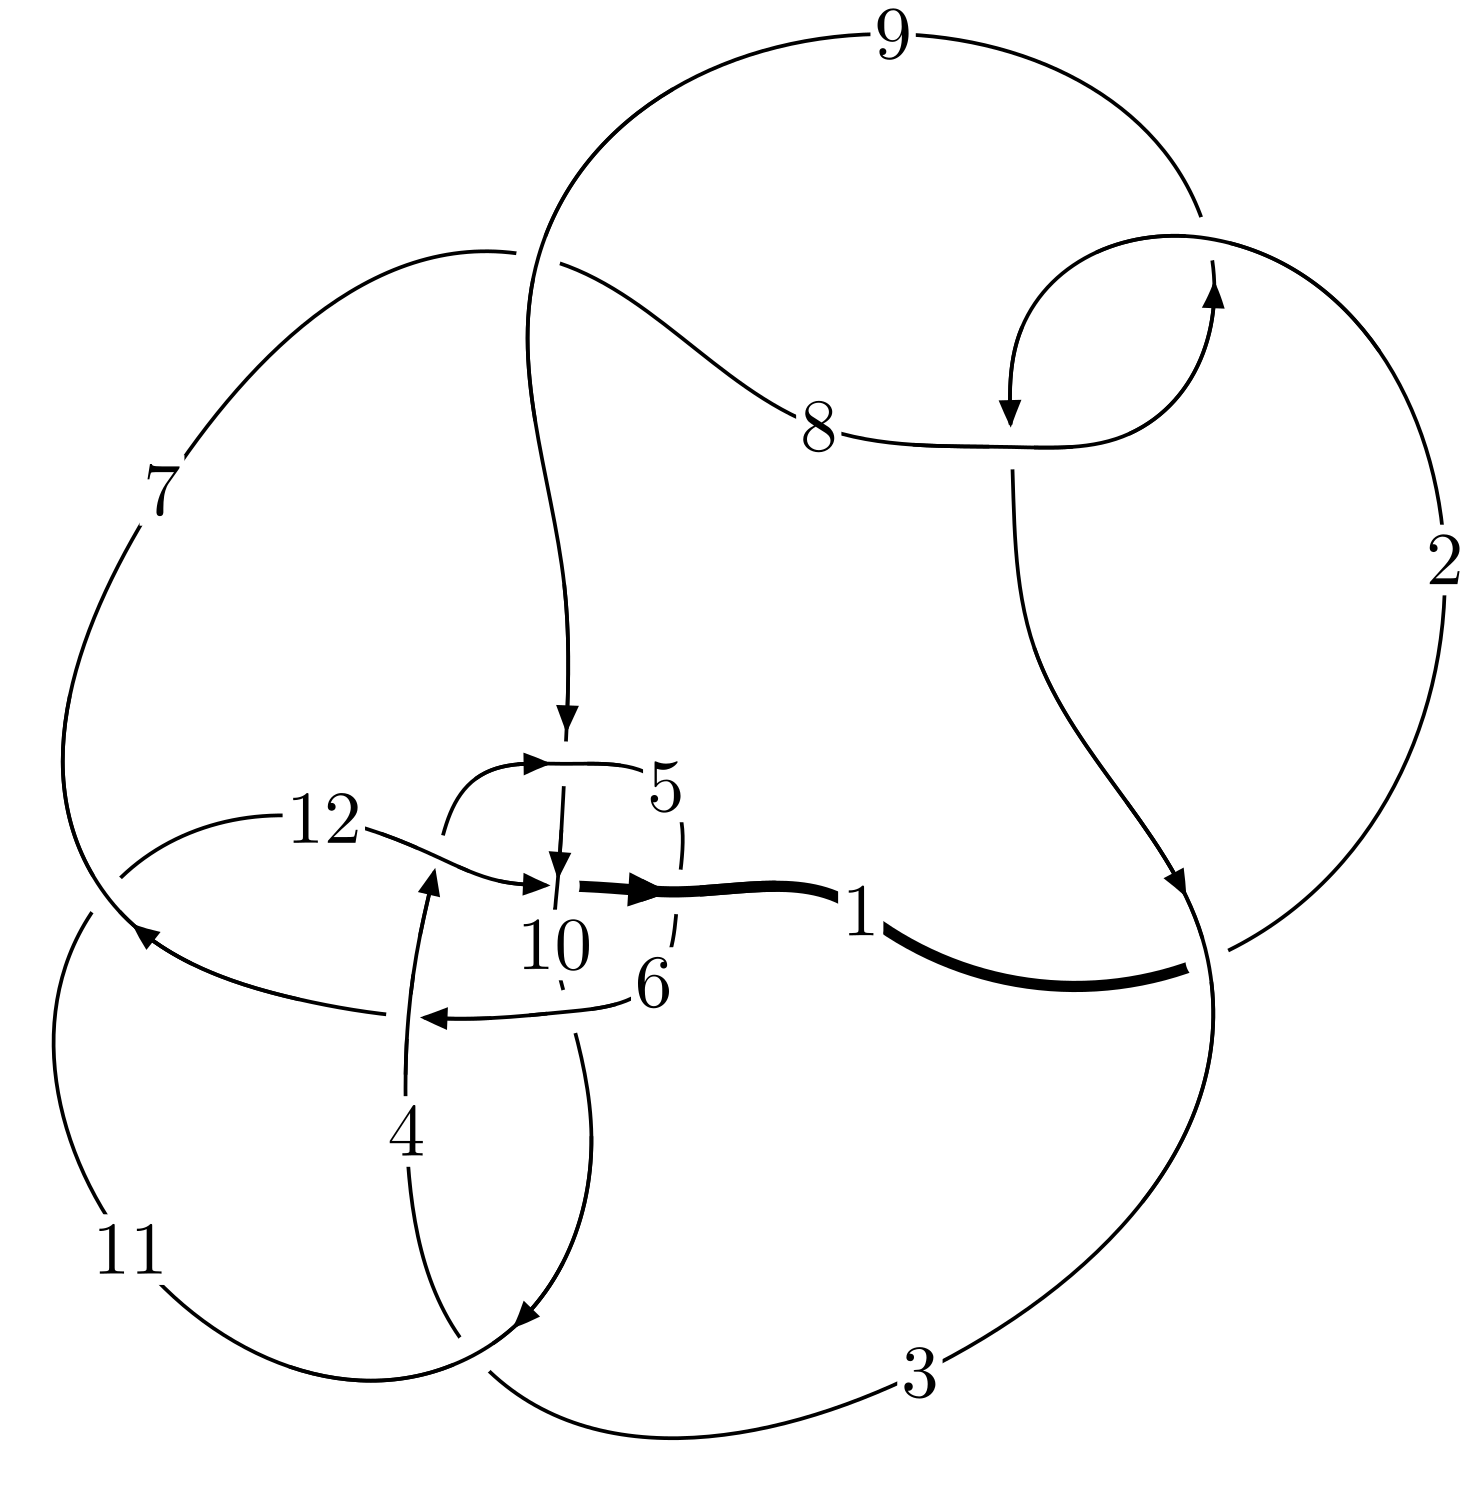
\includegraphics[width=112pt]{../../../GIT/diagram.site/Diagrams/png/1594_12a_0793.png}\\
\ \ \ A knot diagram\footnotemark}&
\allowdisplaybreaks
\textbf{Linearized knot diagam} \\
\cline{2-2}
 &
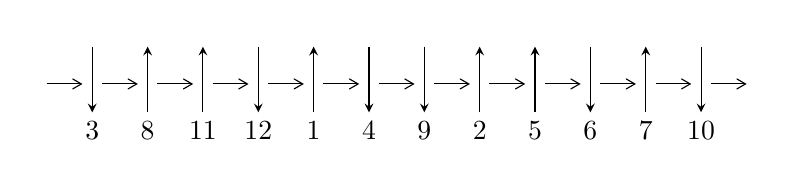
\begin{tikzpicture}[x=20pt, y=17pt]
	% nodes
	\node (C0) at (0, 0) {};
	\node (C1) at (1, 0) {};
	\node (C1U) at (1, +1) {};
	\node (C1D) at (1, -1) {3};

	\node (C2) at (2, 0) {};
	\node (C2U) at (2, +1) {};
	\node (C2D) at (2, -1) {8};

	\node (C3) at (3, 0) {};
	\node (C3U) at (3, +1) {};
	\node (C3D) at (3, -1) {11};

	\node (C4) at (4, 0) {};
	\node (C4U) at (4, +1) {};
	\node (C4D) at (4, -1) {12};

	\node (C5) at (5, 0) {};
	\node (C5U) at (5, +1) {};
	\node (C5D) at (5, -1) {1};

	\node (C6) at (6, 0) {};
	\node (C6U) at (6, +1) {};
	\node (C6D) at (6, -1) {4};

	\node (C7) at (7, 0) {};
	\node (C7U) at (7, +1) {};
	\node (C7D) at (7, -1) {9};

	\node (C8) at (8, 0) {};
	\node (C8U) at (8, +1) {};
	\node (C8D) at (8, -1) {2};

	\node (C9) at (9, 0) {};
	\node (C9U) at (9, +1) {};
	\node (C9D) at (9, -1) {5};

	\node (C10) at (10, 0) {};
	\node (C10U) at (10, +1) {};
	\node (C10D) at (10, -1) {6};

	\node (C11) at (11, 0) {};
	\node (C11U) at (11, +1) {};
	\node (C11D) at (11, -1) {7};

	\node (C12) at (12, 0) {};
	\node (C12U) at (12, +1) {};
	\node (C12D) at (12, -1) {10};
	\node (C13) at (13, 0) {};

	% arrows
	\draw[->,>={angle 60}]
	(C0) edge (C1) (C1) edge (C2) (C2) edge (C3) (C3) edge (C4) (C4) edge (C5) (C5) edge (C6) (C6) edge (C7) (C7) edge (C8) (C8) edge (C9) (C9) edge (C10) (C10) edge (C11) (C11) edge (C12) (C12) edge (C13) ;	\draw[->,>=stealth]
	(C1U) edge (C1D) (C2D) edge (C2U) (C3D) edge (C3U) (C4U) edge (C4D) (C5D) edge (C5U) (C6U) edge (C6D) (C7U) edge (C7D) (C8D) edge (C8U) (C9D) edge (C9U) (C10U) edge (C10D) (C11D) edge (C11U) (C12U) edge (C12D) ;
	\end{tikzpicture} \\
\hhline{~~} \\& 
\textbf{Solving Sequence} \\ \cline{2-2} 
 &
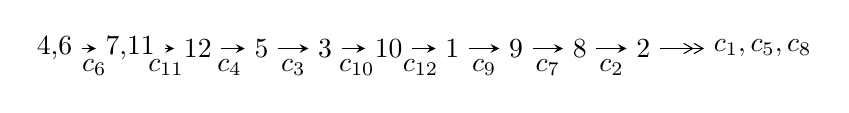
\begin{tikzpicture}[x=23pt, y=7pt]
	% node
	\node (A0) at (-1/8, 0) {4,6};
	\node (A1) at (17/16, 0) {7,11};
	\node (A2) at (17/8, 0) {12};
	\node (A3) at (25/8, 0) {5};
	\node (A4) at (33/8, 0) {3};
	\node (A5) at (41/8, 0) {10};
	\node (A6) at (49/8, 0) {1};
	\node (A7) at (57/8, 0) {9};
	\node (A8) at (65/8, 0) {8};
	\node (A9) at (73/8, 0) {2};
	\node (C1) at (1/2, -1) {$c_{6}$};
	\node (C2) at (13/8, -1) {$c_{11}$};
	\node (C3) at (21/8, -1) {$c_{4}$};
	\node (C4) at (29/8, -1) {$c_{3}$};
	\node (C5) at (37/8, -1) {$c_{10}$};
	\node (C6) at (45/8, -1) {$c_{12}$};
	\node (C7) at (53/8, -1) {$c_{9}$};
	\node (C8) at (61/8, -1) {$c_{7}$};
	\node (C9) at (69/8, -1) {$c_{2}$};
	\node (A10) at (11, 0) {$c_{1},c_{5},c_{8}$};

	% edge
	\draw[->,>=stealth]	
	(A0) edge (A1) (A1) edge (A2) (A2) edge (A3) (A3) edge (A4) (A4) edge (A5) (A5) edge (A6) (A6) edge (A7) (A7) edge (A8) (A8) edge (A9) ;
	\draw[->>,>={angle 60}]	
	(A9) edge (A10);
\end{tikzpicture} \\ 

\end{tabular} \\

\footnotetext{
The image of knot diagram is generated by the software ``\textbf{Draw programme}" developed by Andrew Bartholomew(\url{http://www.layer8.co.uk/maths/draw/index.htm\#Running-draw}), where we modified some parts for our purpose(\url{https://github.com/CATsTAILs/LinksPainter}).
}\phantom \\ \newline 
\centering \textbf{Ideals for irreducible components\footnotemark of $X_{\text{par}}$} 
 
\begin{align*}
I^u_{1}&=\langle 
438 u^{26}-7373 u^{25}+\cdots+b-5644,\;-57808 u^{26}+1046188 u^{25}+\cdots+161 a+5545308,\\
\phantom{I^u_{1}}&\phantom{= \langle  }u^{27}-19 u^{26}+\cdots-2467 u+161\rangle \\
I^u_{2}&=\langle 
10 u^{19}-138 u^{18}+\cdots+b+3377,\;-19597 u^{19}+310175 u^{18}+\cdots+547 a+6609401,\\
\phantom{I^u_{2}}&\phantom{= \langle  }u^{20}-17 u^{19}+\cdots-5470 u+547\rangle \\
I^u_{3}&=\langle 
-2.10186\times10^{16} a^{17} u-3.95962\times10^{16} a^{16} u+\cdots-8.49848\times10^{16} a+1.61926\times10^{17},\\
\phantom{I^u_{3}}&\phantom{= \langle  }a^{17} u+6 a^{16} u+\cdots-4 a-1,\;u^2+u+1\rangle \\
I^u_{4}&=\langle 
-1.67412\times10^{56} a^{17} u^{3}+5.44170\times10^{55} a^{16} u^{3}+\cdots-7.19011\times10^{55} a+1.87024\times10^{54},\\
\phantom{I^u_{4}}&\phantom{= \langle  }4 a^{17} u^3-7 a^{16} u^3+\cdots+13417 a+5031,\;u^4+u^3-2 u+1\rangle \\
I^u_{5}&=\langle 
-6.08618\times10^{26} u^{37}-1.06034\times10^{28} u^{36}+\cdots+4.67445\times10^{25} b-8.22006\times10^{26},\\
\phantom{I^u_{5}}&\phantom{= \langle  }2.32508\times10^{27} u^{37}+4.03483\times10^{28} u^{36}+\cdots+4.67445\times10^{25} a+3.83085\times10^{27},\;u^{38}+18 u^{37}+\cdots-8 u^2+1\rangle \\
I^u_{6}&=\langle 
161661572437 a^{17}+109385111613 b+\cdots+483678202596 a+63623157951,\\
\phantom{I^u_{6}}&\phantom{= \langle  }a^{18}- a^{17}+\cdots+2 a+1,\;u+1\rangle \\
I^u_{7}&=\langle 
b+u,\;a- u,\;u^2+u+1\rangle \\
\\
I^v_{1}&=\langle 
a,\;b^9+b^8-2 b^7-3 b^6+b^5+3 b^4+2 b^3- b-1,\;v-1\rangle \\
\end{align*}
\raggedright * 8 irreducible components of $\dim_{\mathbb{C}}=0$, with total 222 representations.\\
\footnotetext{All coefficients of polynomials are rational numbers. But the coefficients are sometimes approximated in decimal forms when there is not enough margin.}
\newpage
\renewcommand{\arraystretch}{1}
\centering \section*{I. $I^u_{1}= \langle 438 u^{26}-7373 u^{25}+\cdots+b-5644,\;-5.78\times10^{4} u^{26}+1.05\times10^{6} u^{25}+\cdots+161 a+5.55\times10^{6},\;u^{27}-19 u^{26}+\cdots-2467 u+161 \rangle$}
\flushleft \textbf{(i) Arc colorings}\\
\begin{tabular}{m{7pt} m{180pt} m{7pt} m{180pt} }
\flushright $a_{4}=$&$\begin{pmatrix}0\\u\end{pmatrix}$ \\
\flushright $a_{6}=$&$\begin{pmatrix}1\\0\end{pmatrix}$ \\
\flushright $a_{7}=$&$\begin{pmatrix}1\\u^2\end{pmatrix}$ \\
\flushright $a_{11}=$&$\begin{pmatrix}359.056 u^{26}-6498.06 u^{25}+\cdots+518090. u-34442.9\\-438 u^{26}+7373 u^{25}+\cdots-109848 u+5644\end{pmatrix}$ \\
\flushright $a_{12}=$&$\begin{pmatrix}35.0559 u^{26}-228.062 u^{25}+\cdots-333258. u+23365.1\\625 u^{26}-10590 u^{25}+\cdots+223554 u-12710\end{pmatrix}$ \\
\flushright $a_{5}=$&$\begin{pmatrix}0.503106 u^{26}-8.55901 u^{25}+\cdots+85.1429 u-7.16149\\u^{26}-18 u^{25}+\cdots+1234 u-80\end{pmatrix}$ \\
\flushright $a_{3}=$&$\begin{pmatrix}-0.496894 u^{26}+8.44099 u^{25}+\cdots+4.14286 u-8.16149\\u^{25}-17 u^{24}+\cdots-1152 u+81\end{pmatrix}$ \\
\flushright $a_{10}=$&$\begin{pmatrix}-78.9441 u^{26}+874.938 u^{25}+\cdots+408242. u-28798.9\\-438 u^{26}+7373 u^{25}+\cdots-109848 u+5644\end{pmatrix}$ \\
\flushright $a_{1}=$&$\begin{pmatrix}-589.944 u^{26}+10361.9 u^{25}+\cdots-556812. u+36075.1\\-324 u^{26}+6270 u^{25}+\cdots-851348 u+57808\end{pmatrix}$ \\
\flushright $a_{9}=$&$\begin{pmatrix}-217.472 u^{26}+4474.97 u^{25}+\cdots-831411. u+56923.5\\854 u^{26}-14673 u^{25}+\cdots+485474 u-29861\end{pmatrix}$ \\
\flushright $a_{8}=$&$\begin{pmatrix}3.87578 u^{26}-105.640 u^{25}+\cdots+43768.3 u-3039.54\\-42 u^{26}+713 u^{25}+\cdots-9810 u+463\end{pmatrix}$ \\
\flushright $a_{2}=$&$\begin{pmatrix}190.292 u^{26}-4012.55 u^{25}+\cdots+828459. u-56867.2\\-847 u^{26}+14620 u^{25}+\cdots-547319 u+34179\end{pmatrix}$\\&\end{tabular}
\flushleft \textbf{(ii) Obstruction class $= -1$}\\~\\
\flushleft \textbf{(iii) Cusp Shapes $= 572 u^{26}-10814 u^{25}+\cdots+1256842 u-84866$}\\~\\
\newpage\renewcommand{\arraystretch}{1}
\flushleft \textbf{(iv) u-Polynomials at the component}\newline \\
\begin{tabular}{m{50pt}|m{274pt}}
Crossings & \hspace{64pt}u-Polynomials at each crossing \\
\hline $$\begin{aligned}c_{1},c_{7}\end{aligned}$$&$\begin{aligned}
&u^{27}+10 u^{26}+\cdots+208 u-64
\end{aligned}$\\
\hline $$\begin{aligned}c_{2},c_{8}\end{aligned}$$&$\begin{aligned}
&u^{27}+6 u^{26}+\cdots+20 u+8
\end{aligned}$\\
\hline $$\begin{aligned}c_{3},c_{5},c_{9}\\c_{11}\end{aligned}$$&$\begin{aligned}
&u^{27}- u^{26}+\cdots- u+1
\end{aligned}$\\
\hline $$\begin{aligned}c_{4},c_{10}\end{aligned}$$&$\begin{aligned}
&u^{27}+2 u^{26}+\cdots- u-4
\end{aligned}$\\
\hline $$\begin{aligned}c_{6},c_{12}\end{aligned}$$&$\begin{aligned}
&u^{27}-19 u^{26}+\cdots-2467 u+161
\end{aligned}$\\
\hline
\end{tabular}\\~\\
\newpage\renewcommand{\arraystretch}{1}
\flushleft \textbf{(v) Riley Polynomials at the component}\newline \\
\begin{tabular}{m{50pt}|m{274pt}}
Crossings & \hspace{64pt}Riley Polynomials at each crossing \\
\hline $$\begin{aligned}c_{1},c_{7}\end{aligned}$$&$\begin{aligned}
&y^{27}+14 y^{26}+\cdots+92416 y-4096
\end{aligned}$\\
\hline $$\begin{aligned}c_{2},c_{8}\end{aligned}$$&$\begin{aligned}
&y^{27}+10 y^{26}+\cdots+208 y-64
\end{aligned}$\\
\hline $$\begin{aligned}c_{3},c_{5},c_{9}\\c_{11}\end{aligned}$$&$\begin{aligned}
&y^{27}-11 y^{26}+\cdots+35 y-1
\end{aligned}$\\
\hline $$\begin{aligned}c_{4},c_{10}\end{aligned}$$&$\begin{aligned}
&y^{27}-16 y^{26}+\cdots+353 y-16
\end{aligned}$\\
\hline $$\begin{aligned}c_{6},c_{12}\end{aligned}$$&$\begin{aligned}
&y^{27}-19 y^{26}+\cdots+1457339 y-25921
\end{aligned}$\\
\hline
\end{tabular}\\~\\
\newpage\flushleft \textbf{(vi) Complex Volumes and Cusp Shapes}
$$\begin{array}{c|c|c}  
\text{Solutions to }I^u_{1}& \I (\text{vol} + \sqrt{-1}CS) & \text{Cusp shape}\\
 \hline 
\begin{aligned}
u &= \phantom{-}0.336537 + 0.836798 I \\
a &= \phantom{-}0.736010 - 0.616080 I \\
b &= -0.848254 + 0.367605 I\end{aligned}
 & \phantom{-}2.86929 + 7.34613 I & \phantom{-}2.90775 - 7.28964 I \\ \hline\begin{aligned}
u &= \phantom{-}0.336537 - 0.836798 I \\
a &= \phantom{-}0.736010 + 0.616080 I \\
b &= -0.848254 - 0.367605 I\end{aligned}
 & \phantom{-}2.86929 - 7.34613 I & \phantom{-}2.90775 + 7.28964 I \\ \hline\begin{aligned}
u &= -1.10919\phantom{ +0.000000I} \\
a &= -0.386233\phantom{ +0.000000I} \\
b &= -0.903587\phantom{ +0.000000I}\end{aligned}
 & -2.13154\phantom{ +0.000000I} & \phantom{-0.000000 } 0 \\ \hline\begin{aligned}
u &= \phantom{-}0.370735 + 0.693916 I \\
a &= -0.865324 + 0.727255 I \\
b &= \phantom{-}0.749010 - 0.364611 I\end{aligned}
 & \phantom{-}3.95268 + 1.67314 I & \phantom{-}5.49448 - 1.76320 I \\ \hline\begin{aligned}
u &= \phantom{-}0.370735 - 0.693916 I \\
a &= -0.865324 - 0.727255 I \\
b &= \phantom{-}0.749010 + 0.364611 I\end{aligned}
 & \phantom{-}3.95268 - 1.67314 I & \phantom{-}5.49448 + 1.76320 I \\ \hline\begin{aligned}
u &= -0.268476 + 0.625946 I \\
a &= -0.083820 - 0.885103 I \\
b &= -0.847216 + 0.126003 I\end{aligned}
 & -1.73737 + 1.71478 I & -1.17961 - 4.95117 I \\ \hline\begin{aligned}
u &= -0.268476 - 0.625946 I \\
a &= -0.083820 + 0.885103 I \\
b &= -0.847216 - 0.126003 I\end{aligned}
 & -1.73737 - 1.71478 I & -1.17961 + 4.95117 I \\ \hline\begin{aligned}
u &= \phantom{-}1.24557 + 0.71757 I \\
a &= -0.595551 + 0.624978 I \\
b &= -0.544229 - 0.767881 I\end{aligned}
 & \phantom{-}6.27419 - 3.10868 I & \phantom{-0.000000 } 0 \\ \hline\begin{aligned}
u &= \phantom{-}1.24557 - 0.71757 I \\
a &= -0.595551 - 0.624978 I \\
b &= -0.544229 + 0.767881 I\end{aligned}
 & \phantom{-}6.27419 + 3.10868 I & \phantom{-0.000000 } 0 \\ \hline\begin{aligned}
u &= \phantom{-}1.46415\phantom{ +0.000000I} \\
a &= -0.619509\phantom{ +0.000000I} \\
b &= -0.421012\phantom{ +0.000000I}\end{aligned}
 & \phantom{-}0.177089\phantom{ +0.000000I} & \phantom{-0.000000 } 0\\
 \hline 
 \end{array}$$\newpage$$\begin{array}{c|c|c}  
\text{Solutions to }I^u_{1}& \I (\text{vol} + \sqrt{-1}CS) & \text{Cusp shape}\\
 \hline 
\begin{aligned}
u &= \phantom{-}1.24952 + 0.79090 I \\
a &= \phantom{-}0.525687 - 0.707434 I \\
b &= \phantom{-}0.673803 + 0.845192 I\end{aligned}
 & \phantom{-}6.16267 - 9.49500 I & \phantom{-0.000000 } 0 \\ \hline\begin{aligned}
u &= \phantom{-}1.24952 - 0.79090 I \\
a &= \phantom{-}0.525687 + 0.707434 I \\
b &= \phantom{-}0.673803 - 0.845192 I\end{aligned}
 & \phantom{-}6.16267 + 9.49500 I & \phantom{-0.000000 } 0 \\ \hline\begin{aligned}
u &= -1.47651 + 0.36572 I \\
a &= \phantom{-}0.227999 + 0.088281 I \\
b &= \phantom{-}0.930830 - 0.018614 I\end{aligned}
 & -5.14690 + 3.89427 I & \phantom{-0.000000 } 0 \\ \hline\begin{aligned}
u &= -1.47651 - 0.36572 I \\
a &= \phantom{-}0.227999 - 0.088281 I \\
b &= \phantom{-}0.930830 + 0.018614 I\end{aligned}
 & -5.14690 - 3.89427 I & \phantom{-0.000000 } 0 \\ \hline\begin{aligned}
u &= \phantom{-}1.16750 + 1.01896 I \\
a &= -0.058356 + 1.102740 I \\
b &= -1.45088 - 1.00868 I\end{aligned}
 & \phantom{-}0.3619 - 21.2108 I & \phantom{-0.000000 } 0 \\ \hline\begin{aligned}
u &= \phantom{-}1.16750 - 1.01896 I \\
a &= -0.058356 - 1.102740 I \\
b &= -1.45088 + 1.00868 I\end{aligned}
 & \phantom{-}0.3619 + 21.2108 I & \phantom{-0.000000 } 0 \\ \hline\begin{aligned}
u &= \phantom{-}1.17572 + 1.01054 I \\
a &= \phantom{-}0.096238 - 1.077870 I \\
b &= \phantom{-}1.39364 + 1.00946 I\end{aligned}
 & \phantom{-}1.5557 - 15.1733 I & \phantom{-0.000000 } 0 \\ \hline\begin{aligned}
u &= \phantom{-}1.17572 - 1.01054 I \\
a &= \phantom{-}0.096238 + 1.077870 I \\
b &= \phantom{-}1.39364 - 1.00946 I\end{aligned}
 & \phantom{-}1.5557 + 15.1733 I & \phantom{-0.000000 } 0 \\ \hline\begin{aligned}
u &= \phantom{-}1.20645 + 1.03913 I \\
a &= -0.029811 + 0.956551 I \\
b &= -1.37963 - 0.83840 I\end{aligned}
 & -5.7698 - 14.5930 I & \phantom{-0.000000 } 0 \\ \hline\begin{aligned}
u &= \phantom{-}1.20645 - 1.03913 I \\
a &= -0.029811 - 0.956551 I \\
b &= -1.37963 + 0.83840 I\end{aligned}
 & -5.7698 + 14.5930 I & \phantom{-0.000000 } 0\\
 \hline 
 \end{array}$$\newpage$$\begin{array}{c|c|c}  
\text{Solutions to }I^u_{1}& \I (\text{vol} + \sqrt{-1}CS) & \text{Cusp shape}\\
 \hline 
\begin{aligned}
u &= \phantom{-}1.24077 + 1.00164 I \\
a &= \phantom{-}0.145799 - 0.888216 I \\
b &= \phantom{-}1.21535 + 0.84214 I\end{aligned}
 & -1.11103 - 11.43690 I & \phantom{-0.000000 } 0 \\ \hline\begin{aligned}
u &= \phantom{-}1.24077 - 1.00164 I \\
a &= \phantom{-}0.145799 + 0.888216 I \\
b &= \phantom{-}1.21535 - 0.84214 I\end{aligned}
 & -1.11103 + 11.43690 I & \phantom{-0.000000 } 0 \\ \hline\begin{aligned}
u &= \phantom{-}1.29979 + 1.03028 I \\
a &= -0.105556 + 0.759404 I \\
b &= -1.180600 - 0.684143 I\end{aligned}
 & -4.06736 - 6.77038 I & \phantom{-0.000000 } 0 \\ \hline\begin{aligned}
u &= \phantom{-}1.29979 - 1.03028 I \\
a &= -0.105556 - 0.759404 I \\
b &= -1.180600 + 0.684143 I\end{aligned}
 & -4.06736 + 6.77038 I & \phantom{-0.000000 } 0 \\ \hline\begin{aligned}
u &= \phantom{-}1.70957 + 0.33451 I \\
a &= \phantom{-}0.443467 - 0.165713 I \\
b &= \phantom{-}0.622434 + 0.176394 I\end{aligned}
 & -3.79012 - 4.61907 I & \phantom{-0.000000 } 0 \\ \hline\begin{aligned}
u &= \phantom{-}1.70957 - 0.33451 I \\
a &= \phantom{-}0.443467 + 0.165713 I \\
b &= \phantom{-}0.622434 - 0.176394 I\end{aligned}
 & -3.79012 + 4.61907 I & \phantom{-0.000000 } 0 \\ \hline\begin{aligned}
u &= \phantom{-}0.130692\phantom{ +0.000000I} \\
a &= -5.77466\phantom{ +0.000000I} \\
b &= \phantom{-}0.656068\phantom{ +0.000000I}\end{aligned}
 & \phantom{-}1.20181\phantom{ +0.000000I} & \phantom{-}8.52320\phantom{ +0.000000I}\\
 \hline 
 \end{array}$$\newpage\newpage\renewcommand{\arraystretch}{1}
\centering \section*{II. $I^u_{2}= \langle 10 u^{19}-138 u^{18}+\cdots+b+3377,\;-1.96\times10^{4} u^{19}+3.10\times10^{5} u^{18}+\cdots+547 a+6.61\times10^{6},\;u^{20}-17 u^{19}+\cdots-5470 u+547 \rangle$}
\flushleft \textbf{(i) Arc colorings}\\
\begin{tabular}{m{7pt} m{180pt} m{7pt} m{180pt} }
\flushright $a_{4}=$&$\begin{pmatrix}0\\u\end{pmatrix}$ \\
\flushright $a_{6}=$&$\begin{pmatrix}1\\0\end{pmatrix}$ \\
\flushright $a_{7}=$&$\begin{pmatrix}1\\u^2\end{pmatrix}$ \\
\flushright $a_{11}=$&$\begin{pmatrix}35.8263 u^{19}-567.048 u^{18}+\cdots+116532. u-12083\\-10 u^{19}+138 u^{18}+\cdots+26256 u-3377\end{pmatrix}$ \\
\flushright $a_{12}=$&$\begin{pmatrix}-6.17367 u^{19}+114.952 u^{18}+\cdots-67354.8 u+7514\\-10 u^{19}+189 u^{18}+\cdots-125810 u+14127\end{pmatrix}$ \\
\flushright $a_{5}=$&$\begin{pmatrix}-0.500914 u^{19}+7.51554 u^{18}+\cdots-161.757 u+5\\- u^{19}+16 u^{18}+\cdots-2734 u+273\end{pmatrix}$ \\
\flushright $a_{3}=$&$\begin{pmatrix}1.49909 u^{19}-23.4845 u^{18}+\cdots+5036.24 u-541\\- u^{18}+15 u^{17}+\cdots+2462 u-274\end{pmatrix}$ \\
\flushright $a_{10}=$&$\begin{pmatrix}25.8263 u^{19}-429.048 u^{18}+\cdots+142788. u-15460\\-10 u^{19}+138 u^{18}+\cdots+26256 u-3377\end{pmatrix}$ \\
\flushright $a_{1}=$&$\begin{pmatrix}58.8263 u^{19}-915.048 u^{18}+\cdots+140957. u-13914\\22 u^{19}-355 u^{18}+\cdots+84333 u-8847\end{pmatrix}$ \\
\flushright $a_{9}=$&$\begin{pmatrix}34.2395 u^{19}-584.071 u^{18}+\cdots+235307. u-25699\\-19 u^{19}+272 u^{18}+\cdots+34877 u-4792\end{pmatrix}$ \\
\flushright $a_{8}=$&$\begin{pmatrix}0.372943 u^{19}+3.65996 u^{18}+\cdots-26140.2 u+2952\\8 u^{19}-122 u^{18}+\cdots+5813 u-343\end{pmatrix}$ \\
\flushright $a_{2}=$&$\begin{pmatrix}-33.5539 u^{19}+582.417 u^{18}+\cdots-260246. u+28513\\28 u^{19}-421 u^{18}+\cdots+12884 u-303\end{pmatrix}$\\&\end{tabular}
\flushleft \textbf{(ii) Obstruction class $= -1$}\\~\\
\flushleft \textbf{(iii) Cusp Shapes $= -74 u^{19}+1205 u^{18}-10121 u^{17}+57171 u^{16}-241507 u^{15}+807130 u^{14}-2208198 u^{13}+5054483 u^{12}-9813175 u^{11}+16283515 u^{10}-23153095 u^9+28154252 u^8-29094801 u^7+25274749 u^6-18155481 u^5+10525995 u^4-4748224 u^3+1569915 u^2-340234 u+36612$}\\~\\
\newpage\renewcommand{\arraystretch}{1}
\flushleft \textbf{(iv) u-Polynomials at the component}\newline \\
\begin{tabular}{m{50pt}|m{274pt}}
Crossings & \hspace{64pt}u-Polynomials at each crossing \\
\hline $$\begin{aligned}c_{1},c_{7}\end{aligned}$$&$\begin{aligned}
&(u^{10}+3 u^9+\cdots+4 u+16)^{2}
\end{aligned}$\\
\hline $$\begin{aligned}c_{2},c_{8}\end{aligned}$$&$\begin{aligned}
&(u^{10}+3 u^9+6 u^8+7 u^7+7 u^6+4 u^5+2 u^4+u^3+5 u^2+6 u+4)^2
\end{aligned}$\\
\hline $$\begin{aligned}c_{3},c_{5},c_{9}\\c_{11}\end{aligned}$$&$\begin{aligned}
&u^{20}+u^{19}+\cdots+4 u+1
\end{aligned}$\\
\hline $$\begin{aligned}c_{4},c_{10}\end{aligned}$$&$\begin{aligned}
&(u^{10}- u^9+2 u^8-2 u^7+3 u^6-2 u^5+4 u^4-3 u^3+2 u^2- u+1)^2
\end{aligned}$\\
\hline $$\begin{aligned}c_{6},c_{12}\end{aligned}$$&$\begin{aligned}
&u^{20}-17 u^{19}+\cdots-5470 u+547
\end{aligned}$\\
\hline
\end{tabular}\\~\\
\newpage\renewcommand{\arraystretch}{1}
\flushleft \textbf{(v) Riley Polynomials at the component}\newline \\
\begin{tabular}{m{50pt}|m{274pt}}
Crossings & \hspace{64pt}Riley Polynomials at each crossing \\
\hline $$\begin{aligned}c_{1},c_{7}\end{aligned}$$&$\begin{aligned}
&(y^{10}+7 y^9+\cdots+912 y+256)^{2}
\end{aligned}$\\
\hline $$\begin{aligned}c_{2},c_{8}\end{aligned}$$&$\begin{aligned}
&(y^{10}+3 y^9+\cdots+4 y+16)^{2}
\end{aligned}$\\
\hline $$\begin{aligned}c_{3},c_{5},c_{9}\\c_{11}\end{aligned}$$&$\begin{aligned}
&y^{20}-3 y^{19}+\cdots-6 y+1
\end{aligned}$\\
\hline $$\begin{aligned}c_{4},c_{10}\end{aligned}$$&$\begin{aligned}
&(y^{10}+3 y^9+6 y^8+12 y^7+15 y^6+16 y^5+16 y^4+9 y^3+6 y^2+3 y+1)^2
\end{aligned}$\\
\hline $$\begin{aligned}c_{6},c_{12}\end{aligned}$$&$\begin{aligned}
&y^{20}+9 y^{19}+\cdots-291004 y+299209
\end{aligned}$\\
\hline
\end{tabular}\\~\\
\newpage\flushleft \textbf{(vi) Complex Volumes and Cusp Shapes}
$$\begin{array}{c|c|c}  
\text{Solutions to }I^u_{2}& \I (\text{vol} + \sqrt{-1}CS) & \text{Cusp shape}\\
 \hline 
\begin{aligned}
u &= \phantom{-}0.677518 + 0.918459 I \\
a &= -0.283415 + 1.066980 I \\
b &= -0.046924 - 1.225610 I\end{aligned}
 & \phantom{-}8.01878 - 3.00602 I & \phantom{-}7.09865 + 2.87547 I \\ \hline\begin{aligned}
u &= \phantom{-}0.677518 - 0.918459 I \\
a &= -0.283415 - 1.066980 I \\
b &= -0.046924 + 1.225610 I\end{aligned}
 & \phantom{-}8.01878 + 3.00602 I & \phantom{-}7.09865 - 2.87547 I \\ \hline\begin{aligned}
u &= \phantom{-}0.659672 + 0.969287 I \\
a &= \phantom{-}0.299146 - 0.973357 I \\
b &= -0.046924 + 1.225610 I\end{aligned}
 & \phantom{-}8.01878 + 3.00602 I & \phantom{-}7.09865 - 2.87547 I \\ \hline\begin{aligned}
u &= \phantom{-}0.659672 - 0.969287 I \\
a &= \phantom{-}0.299146 + 0.973357 I \\
b &= -0.046924 - 1.225610 I\end{aligned}
 & \phantom{-}8.01878 - 3.00602 I & \phantom{-}7.09865 + 2.87547 I \\ \hline\begin{aligned}
u &= \phantom{-}0.701824 + 0.417724 I \\
a &= -0.12548 + 1.75109 I \\
b &= -0.247103 - 0.693158 I\end{aligned}
 & \phantom{-}1.22482 - 2.54559 I & \phantom{-}8.96438 - 3.81169 I \\ \hline\begin{aligned}
u &= \phantom{-}0.701824 - 0.417724 I \\
a &= -0.12548 - 1.75109 I \\
b &= -0.247103 + 0.693158 I\end{aligned}
 & \phantom{-}1.22482 + 2.54559 I & \phantom{-}8.96438 + 3.81169 I \\ \hline\begin{aligned}
u &= \phantom{-}0.997260 + 0.676475 I \\
a &= -0.259742 + 1.345110 I \\
b &= -0.785372 - 0.793969 I\end{aligned}
 & \phantom{-}2.56812 - 6.71853 I & \phantom{-0.000000 -}0. + 9.04516 I \\ \hline\begin{aligned}
u &= \phantom{-}0.997260 - 0.676475 I \\
a &= -0.259742 - 1.345110 I \\
b &= -0.785372 + 0.793969 I\end{aligned}
 & \phantom{-}2.56812 + 6.71853 I & \phantom{-0.000000 } 0. - 9.04516 I \\ \hline\begin{aligned}
u &= \phantom{-}1.112530 + 0.520031 I \\
a &= \phantom{-}0.473491 - 1.197620 I \\
b &= \phantom{-}0.694203 + 0.475585 I\end{aligned}
 & -4.79509 - 5.43520 I & -14.2284 + 21.7220 I \\ \hline\begin{aligned}
u &= \phantom{-}1.112530 - 0.520031 I \\
a &= \phantom{-}0.473491 + 1.197620 I \\
b &= \phantom{-}0.694203 - 0.475585 I\end{aligned}
 & -4.79509 + 5.43520 I & -14.2284 - 21.7220 I\\
 \hline 
 \end{array}$$\newpage$$\begin{array}{c|c|c}  
\text{Solutions to }I^u_{2}& \I (\text{vol} + \sqrt{-1}CS) & \text{Cusp shape}\\
 \hline 
\begin{aligned}
u &= \phantom{-}1.030430 + 0.704082 I \\
a &= \phantom{-}0.220528 - 1.322220 I \\
b &= \phantom{-}0.885197 + 0.778729 I\end{aligned}
 & \phantom{-}1.20804 - 12.75960 I & \phantom{-0.000000 -}0. + 12.39712 I \\ \hline\begin{aligned}
u &= \phantom{-}1.030430 - 0.704082 I \\
a &= \phantom{-}0.220528 + 1.322220 I \\
b &= \phantom{-}0.885197 - 0.778729 I\end{aligned}
 & \phantom{-}1.20804 + 12.75960 I & \phantom{-0.000000 } 0. - 12.39712 I \\ \hline\begin{aligned}
u &= -0.13202 + 1.58588 I \\
a &= -0.083726 - 0.222070 I \\
b &= -0.247103 + 0.693158 I\end{aligned}
 & \phantom{-}1.22482 + 2.54559 I & \phantom{-0.000000 } 0 \\ \hline\begin{aligned}
u &= -0.13202 - 1.58588 I \\
a &= -0.083726 + 0.222070 I \\
b &= -0.247103 - 0.693158 I\end{aligned}
 & \phantom{-}1.22482 - 2.54559 I & \phantom{-0.000000 } 0 \\ \hline\begin{aligned}
u &= \phantom{-}1.06126 + 1.41764 I \\
a &= -0.468889 + 0.016745 I \\
b &= \phantom{-}0.885197 - 0.778729 I\end{aligned}
 & \phantom{-}1.20804 + 12.75960 I & \phantom{-0.000000 } 0 \\ \hline\begin{aligned}
u &= \phantom{-}1.06126 - 1.41764 I \\
a &= -0.468889 - 0.016745 I \\
b &= \phantom{-}0.885197 + 0.778729 I\end{aligned}
 & \phantom{-}1.20804 - 12.75960 I & \phantom{-0.000000 } 0 \\ \hline\begin{aligned}
u &= \phantom{-}0.99401 + 1.47823 I \\
a &= \phantom{-}0.415405 - 0.085464 I \\
b &= -0.785372 + 0.793969 I\end{aligned}
 & \phantom{-}2.56812 + 6.71853 I & \phantom{-0.000000 } 0 \\ \hline\begin{aligned}
u &= \phantom{-}0.99401 - 1.47823 I \\
a &= \phantom{-}0.415405 + 0.085464 I \\
b &= -0.785372 - 0.793969 I\end{aligned}
 & \phantom{-}2.56812 - 6.71853 I & \phantom{-0.000000 } 0 \\ \hline\begin{aligned}
u &= \phantom{-}1.39751 + 1.83694 I \\
a &= -0.187318 - 0.050399 I \\
b &= \phantom{-}0.694203 - 0.475585 I\end{aligned}
 & -4.79509 + 5.43520 I & \phantom{-0.000000 } 0 \\ \hline\begin{aligned}
u &= \phantom{-}1.39751 - 1.83694 I \\
a &= -0.187318 + 0.050399 I \\
b &= \phantom{-}0.694203 + 0.475585 I\end{aligned}
 & -4.79509 - 5.43520 I & \phantom{-0.000000 } 0\\
 \hline 
 \end{array}$$\newpage\newpage\renewcommand{\arraystretch}{1}
\centering \section*{III. $I^u_{3}= \langle -2.10\times10^{16} a^{17} u-3.96\times10^{16} a^{16} u+\cdots-8.50\times10^{16} a+1.62\times10^{17},\;a^{17} u+6 a^{16} u+\cdots-4 a-1,\;u^2+u+1 \rangle$}
\flushleft \textbf{(i) Arc colorings}\\
\begin{tabular}{m{7pt} m{180pt} m{7pt} m{180pt} }
\flushright $a_{4}=$&$\begin{pmatrix}0\\u\end{pmatrix}$ \\
\flushright $a_{6}=$&$\begin{pmatrix}1\\0\end{pmatrix}$ \\
\flushright $a_{7}=$&$\begin{pmatrix}1\\- u-1\end{pmatrix}$ \\
\flushright $a_{11}=$&$\begin{pmatrix}a\\0.0959303 a^{17} u+0.180720 a^{16} u+\cdots+0.387877 a-0.739044\end{pmatrix}$ \\
\flushright $a_{12}=$&$\begin{pmatrix}0.0959303 a^{17} u+0.180720 a^{16} u+\cdots+2.38788 a-0.739044\\-0.461097 a^{17} u+0.273775 a^{16} u+\cdots+5.32003 a+0.717805\end{pmatrix}$ \\
\flushright $a_{5}=$&$\begin{pmatrix}-0.280377 a^{17} u+0.0689210 a^{16} u+\cdots+1.68093 a+1.55703\\- a^2 u- a^2\end{pmatrix}$ \\
\flushright $a_{3}=$&$\begin{pmatrix}- a^2 u\\-0.283253 a^{17} u+0.0132106 a^{16} u+\cdots+0.179332 a+0.0959303\end{pmatrix}$ \\
\flushright $a_{10}=$&$\begin{pmatrix}0.0959303 a^{17} u+0.180720 a^{16} u+\cdots+1.38788 a-0.739044\\0.0959303 a^{17} u+0.180720 a^{16} u+\cdots+0.387877 a-0.739044\end{pmatrix}$ \\
\flushright $a_{1}=$&$\begin{pmatrix}0.557028 a^{17} u-0.0930548 a^{16} u+\cdots-2.93216 a-1.45685\\- a u\end{pmatrix}$ \\
\flushright $a_{9}=$&$\begin{pmatrix}- a^3 u- a^3-2 a u- a\\-0.128737 a^{17} u+0.242628 a^{16} u+\cdots+1.98774 a-0.455792\end{pmatrix}$ \\
\flushright $a_{8}=$&$\begin{pmatrix}0.0478671 a^{17} u-0.111173 a^{16} u+\cdots-2.64693 a+0.379956\\0.369293 a^{17} u+0.00145360 a^{16} u+\cdots-3.00361 a-0.982614\end{pmatrix}$ \\
\flushright $a_{2}=$&$\begin{pmatrix}0.372906 a^{17} u-0.0550592 a^{16} u+\cdots-0.798659 a-1.02405\\-0.616623 a^{17} u+0.469416 a^{16} u+\cdots+0.749763 a+0.122688\end{pmatrix}$\\&\end{tabular}
\flushleft \textbf{(ii) Obstruction class $= -1$}\\~\\
\flushleft \textbf{(iii) Cusp Shapes $= -\frac{670869991029847876}{219102404420358169} a^{17} u+\frac{387999224026686928}{219102404420358169} a^{16} u+\cdots+\frac{7273155080522331304}{219102404420358169} a+\frac{1021136578232313598}{219102404420358169}$}\\~\\
\newpage\renewcommand{\arraystretch}{1}
\flushleft \textbf{(iv) u-Polynomials at the component}\newline \\
\begin{tabular}{m{50pt}|m{274pt}}
Crossings & \hspace{64pt}u-Polynomials at each crossing \\
\hline $$\begin{aligned}c_{1},c_{7}\end{aligned}$$&$\begin{aligned}
&(u^9+3 u^8+8 u^7+13 u^6+17 u^5+17 u^4+12 u^3+6 u^2+u-1)^4
\end{aligned}$\\
\hline $$\begin{aligned}c_{2},c_{8}\end{aligned}$$&$\begin{aligned}
&(u^9- u^8+2 u^7- u^6+3 u^5- u^4+2 u^3+u+1)^4
\end{aligned}$\\
\hline $$\begin{aligned}c_{3},c_{5},c_{9}\\c_{11}\end{aligned}$$&$\begin{aligned}
&u^{36}+u^{35}+\cdots+8 u+1
\end{aligned}$\\
\hline $$\begin{aligned}c_{4},c_{10}\end{aligned}$$&$\begin{aligned}
&u^{36}+3 u^{35}+\cdots+2544 u+889
\end{aligned}$\\
\hline $$\begin{aligned}c_{6},c_{12}\end{aligned}$$&$\begin{aligned}
&(u^2+u+1)^{18}
\end{aligned}$\\
\hline
\end{tabular}\\~\\
\newpage\renewcommand{\arraystretch}{1}
\flushleft \textbf{(v) Riley Polynomials at the component}\newline \\
\begin{tabular}{m{50pt}|m{274pt}}
Crossings & \hspace{64pt}Riley Polynomials at each crossing \\
\hline $$\begin{aligned}c_{1},c_{7}\end{aligned}$$&$\begin{aligned}
&(y^9+7 y^8+20 y^7+25 y^6+5 y^5-15 y^4+22 y^2+13 y-1)^4
\end{aligned}$\\
\hline $$\begin{aligned}c_{2},c_{8}\end{aligned}$$&$\begin{aligned}
&(y^9+3 y^8+8 y^7+13 y^6+17 y^5+17 y^4+12 y^3+6 y^2+y-1)^4
\end{aligned}$\\
\hline $$\begin{aligned}c_{3},c_{5},c_{9}\\c_{11}\end{aligned}$$&$\begin{aligned}
&y^{36}+3 y^{35}+\cdots+24 y+1
\end{aligned}$\\
\hline $$\begin{aligned}c_{4},c_{10}\end{aligned}$$&$\begin{aligned}
&y^{36}+23 y^{35}+\cdots-6905768 y+790321
\end{aligned}$\\
\hline $$\begin{aligned}c_{6},c_{12}\end{aligned}$$&$\begin{aligned}
&(y^2+y+1)^{18}
\end{aligned}$\\
\hline
\end{tabular}\\~\\
\newpage\flushleft \textbf{(vi) Complex Volumes and Cusp Shapes}
$$\begin{array}{c|c|c}  
\text{Solutions to }I^u_{3}& \I (\text{vol} + \sqrt{-1}CS) & \text{Cusp shape}\\
 \hline 
\begin{aligned}
u &= -0.500000 + 0.866025 I \\
a &= -0.230058 - 0.974073 I \\
b &= \phantom{-}0.47792 + 2.18649 I\end{aligned}
 & \phantom{-}4.37135 + 5.39594 I & \phantom{-}7.28409 - 7.62995 I \\ \hline\begin{aligned}
u &= -0.500000 + 0.866025 I \\
a &= -0.059643 + 0.996048 I \\
b &= \phantom{-}0.11516 - 1.92059 I\end{aligned}
 & -1.78344 + 6.15314 I & -0.51499 - 11.09103 I \\ \hline\begin{aligned}
u &= -0.500000 + 0.866025 I \\
a &= \phantom{-}0.134816 - 0.936195 I \\
b &= -0.963253 + 0.522002 I\end{aligned}
 & -1.78344 + 1.96639 I & -0.51499 - 2.76537 I \\ \hline\begin{aligned}
u &= -0.500000 + 0.866025 I \\
a &= \phantom{-}0.206770 + 1.051500 I \\
b &= -0.35966 - 2.31708 I\end{aligned}
 & \phantom{-}3.59813 + 11.14470 I & \phantom{-}5.57680 - 12.84155 I \\ \hline\begin{aligned}
u &= -0.500000 + 0.866025 I \\
a &= \phantom{-}0.437408 - 0.992085 I \\
b &= -1.14872 + 1.23939 I\end{aligned}
 & \phantom{-}0.61694 + 6.51418 I & \phantom{-}2.32792 - 9.84118 I \\ \hline\begin{aligned}
u &= -0.500000 + 0.866025 I \\
a &= -0.374860 + 1.040260 I \\
b &= \phantom{-}0.94469 - 1.53262 I\end{aligned}
 & \phantom{-}0.61694 + 1.60535 I & \phantom{-}2.32792 - 4.01523 I \\ \hline\begin{aligned}
u &= -0.500000 + 0.866025 I \\
a &= -1.007240 + 0.499722 I \\
b &= \phantom{-}0.295924 - 0.252417 I\end{aligned}
 & \phantom{-}0.61694 + 6.51418 I & \phantom{-}2.32792 - 9.84118 I \\ \hline\begin{aligned}
u &= -0.500000 + 0.866025 I \\
a &= \phantom{-}1.086170 - 0.792955 I \\
b &= -0.516345 + 0.300592 I\end{aligned}
 & \phantom{-}0.61694 + 1.60535 I & \phantom{-}2.32792 - 4.01523 I \\ \hline\begin{aligned}
u &= -0.500000 + 0.866025 I \\
a &= \phantom{-}0.007976 - 0.628437 I \\
b &= \phantom{-}0.404990 + 1.343720 I\end{aligned}
 & \phantom{-}1.19845 + 4.05977 I & \phantom{-}8.65235 - 6.92820 I \\ \hline\begin{aligned}
u &= -0.500000 + 0.866025 I \\
a &= -0.420943 + 1.343720 I \\
b &= \phantom{-}0.833909 - 0.628437 I\end{aligned}
 & \phantom{-}1.19845 + 4.05977 I & \phantom{-}8.65235 - 6.92820 I\\
 \hline 
 \end{array}$$\newpage$$\begin{array}{c|c|c}  
\text{Solutions to }I^u_{3}& \I (\text{vol} + \sqrt{-1}CS) & \text{Cusp shape}\\
 \hline 
\begin{aligned}
u &= -0.500000 + 0.866025 I \\
a &= -0.31206 - 1.40188 I \\
b &= -0.707522 + 0.636684 I\end{aligned}
 & \phantom{-}3.59813 - 3.02516 I & \phantom{-}5.57680 - 1.01485 I \\ \hline\begin{aligned}
u &= -0.500000 + 0.866025 I \\
a &= \phantom{-}0.16655 + 1.47381 I \\
b &= \phantom{-}0.759506 - 0.652955 I\end{aligned}
 & \phantom{-}4.37135 + 2.72360 I & \phantom{-}7.28409 - 6.22645 I \\ \hline\begin{aligned}
u &= -0.500000 + 0.866025 I \\
a &= -0.414405 - 0.261400 I \\
b &= \phantom{-}1.34046 + 1.08226 I\end{aligned}
 & \phantom{-}4.37135 + 2.72360 I & \phantom{-}7.28409 - 6.22645 I \\ \hline\begin{aligned}
u &= -0.500000 + 0.866025 I \\
a &= \phantom{-}0.464951 + 0.136300 I \\
b &= -1.48453 - 0.90150 I\end{aligned}
 & \phantom{-}3.59813 - 3.02516 I & \phantom{-}5.57680 - 1.01485 I \\ \hline\begin{aligned}
u &= -0.500000 + 0.866025 I \\
a &= \phantom{-}0.88808 - 1.41024 I \\
b &= -0.832563 + 0.485697 I\end{aligned}
 & -1.78344 + 6.15314 I & -0.51499 - 11.09103 I \\ \hline\begin{aligned}
u &= -0.500000 + 0.866025 I \\
a &= -0.190333 + 0.011651 I \\
b &= -0.638104 - 0.425844 I\end{aligned}
 & -1.78344 + 1.96639 I & -0.51499 - 2.76537 I \\ \hline\begin{aligned}
u &= -0.500000 + 0.866025 I \\
a &= -0.69599 + 1.79493 I \\
b &= \phantom{-}0.943853 - 0.582518 I\end{aligned}
 & \phantom{-}4.37135 + 5.39594 I & \phantom{-}7.28409 - 7.62995 I \\ \hline\begin{aligned}
u &= -0.500000 + 0.866025 I \\
a &= \phantom{-}0.81281 - 1.81670 I \\
b &= -0.965703 + 0.551117 I\end{aligned}
 & \phantom{-}3.59813 + 11.14470 I & \phantom{-}5.57680 - 12.84155 I \\ \hline\begin{aligned}
u &= -0.500000 - 0.866025 I \\
a &= -0.230058 + 0.974073 I \\
b &= \phantom{-}0.47792 - 2.18649 I\end{aligned}
 & \phantom{-}4.37135 - 5.39594 I & \phantom{-}7.28409 + 7.62995 I \\ \hline\begin{aligned}
u &= -0.500000 - 0.866025 I \\
a &= -0.059643 - 0.996048 I \\
b &= \phantom{-}0.11516 + 1.92059 I\end{aligned}
 & -1.78344 - 6.15314 I & -0.51499 + 11.09103 I\\
 \hline 
 \end{array}$$\newpage$$\begin{array}{c|c|c}  
\text{Solutions to }I^u_{3}& \I (\text{vol} + \sqrt{-1}CS) & \text{Cusp shape}\\
 \hline 
\begin{aligned}
u &= -0.500000 - 0.866025 I \\
a &= \phantom{-}0.134816 + 0.936195 I \\
b &= -0.963253 - 0.522002 I\end{aligned}
 & -1.78344 - 1.96639 I & -0.51499 + 2.76537 I \\ \hline\begin{aligned}
u &= -0.500000 - 0.866025 I \\
a &= \phantom{-}0.206770 - 1.051500 I \\
b &= -0.35966 + 2.31708 I\end{aligned}
 & \phantom{-}3.59813 - 11.14470 I & \phantom{-}5.57680 + 12.84155 I \\ \hline\begin{aligned}
u &= -0.500000 - 0.866025 I \\
a &= \phantom{-}0.437408 + 0.992085 I \\
b &= -1.14872 - 1.23939 I\end{aligned}
 & \phantom{-}0.61694 - 6.51418 I & \phantom{-}2.32792 + 9.84118 I \\ \hline\begin{aligned}
u &= -0.500000 - 0.866025 I \\
a &= -0.374860 - 1.040260 I \\
b &= \phantom{-}0.94469 + 1.53262 I\end{aligned}
 & \phantom{-}0.61694 - 1.60535 I & \phantom{-}2.32792 + 4.01523 I \\ \hline\begin{aligned}
u &= -0.500000 - 0.866025 I \\
a &= -1.007240 - 0.499722 I \\
b &= \phantom{-}0.295924 + 0.252417 I\end{aligned}
 & \phantom{-}0.61694 - 6.51418 I & \phantom{-}2.32792 + 9.84118 I \\ \hline\begin{aligned}
u &= -0.500000 - 0.866025 I \\
a &= \phantom{-}1.086170 + 0.792955 I \\
b &= -0.516345 - 0.300592 I\end{aligned}
 & \phantom{-}0.61694 - 1.60535 I & \phantom{-}2.32792 + 4.01523 I \\ \hline\begin{aligned}
u &= -0.500000 - 0.866025 I \\
a &= \phantom{-}0.007976 + 0.628437 I \\
b &= \phantom{-}0.404990 - 1.343720 I\end{aligned}
 & \phantom{-}1.19845 - 4.05977 I & \phantom{-}8.65235 + 6.92820 I \\ \hline\begin{aligned}
u &= -0.500000 - 0.866025 I \\
a &= -0.420943 - 1.343720 I \\
b &= \phantom{-}0.833909 + 0.628437 I\end{aligned}
 & \phantom{-}1.19845 - 4.05977 I & \phantom{-}8.65235 + 6.92820 I \\ \hline\begin{aligned}
u &= -0.500000 - 0.866025 I \\
a &= -0.31206 + 1.40188 I \\
b &= -0.707522 - 0.636684 I\end{aligned}
 & \phantom{-}3.59813 + 3.02516 I & \phantom{-}5.57680 + 1.01485 I \\ \hline\begin{aligned}
u &= -0.500000 - 0.866025 I \\
a &= \phantom{-}0.16655 - 1.47381 I \\
b &= \phantom{-}0.759506 + 0.652955 I\end{aligned}
 & \phantom{-}4.37135 - 2.72360 I & \phantom{-}7.28409 + 6.22645 I\\
 \hline 
 \end{array}$$\newpage$$\begin{array}{c|c|c}  
\text{Solutions to }I^u_{3}& \I (\text{vol} + \sqrt{-1}CS) & \text{Cusp shape}\\
 \hline 
\begin{aligned}
u &= -0.500000 - 0.866025 I \\
a &= -0.414405 + 0.261400 I \\
b &= \phantom{-}1.34046 - 1.08226 I\end{aligned}
 & \phantom{-}4.37135 - 2.72360 I & \phantom{-}7.28409 + 6.22645 I \\ \hline\begin{aligned}
u &= -0.500000 - 0.866025 I \\
a &= \phantom{-}0.464951 - 0.136300 I \\
b &= -1.48453 + 0.90150 I\end{aligned}
 & \phantom{-}3.59813 + 3.02516 I & \phantom{-}5.57680 + 1.01485 I \\ \hline\begin{aligned}
u &= -0.500000 - 0.866025 I \\
a &= \phantom{-}0.88808 + 1.41024 I \\
b &= -0.832563 - 0.485697 I\end{aligned}
 & -1.78344 - 6.15314 I & -0.51499 + 11.09103 I \\ \hline\begin{aligned}
u &= -0.500000 - 0.866025 I \\
a &= -0.190333 - 0.011651 I \\
b &= -0.638104 + 0.425844 I\end{aligned}
 & -1.78344 - 1.96639 I & -0.51499 + 2.76537 I \\ \hline\begin{aligned}
u &= -0.500000 - 0.866025 I \\
a &= -0.69599 - 1.79493 I \\
b &= \phantom{-}0.943853 + 0.582518 I\end{aligned}
 & \phantom{-}4.37135 - 5.39594 I & \phantom{-}7.28409 + 7.62995 I \\ \hline\begin{aligned}
u &= -0.500000 - 0.866025 I \\
a &= \phantom{-}0.81281 + 1.81670 I \\
b &= -0.965703 - 0.551117 I\end{aligned}
 & \phantom{-}3.59813 - 11.14470 I & \phantom{-}5.57680 + 12.84155 I\\
 \hline 
 \end{array}$$\newpage\newpage\renewcommand{\arraystretch}{1}
\centering \section*{IV. $I^u_{4}= \langle -1.67\times10^{56} a^{17} u^{3}+5.44\times10^{55} a^{16} u^{3}+\cdots-7.19\times10^{55} a+1.87\times10^{54},\;4 a^{17} u^3-7 a^{16} u^3+\cdots+13417 a+5031,\;u^4+u^3-2 u+1 \rangle$}
\flushleft \textbf{(i) Arc colorings}\\
\begin{tabular}{m{7pt} m{180pt} m{7pt} m{180pt} }
\flushright $a_{4}=$&$\begin{pmatrix}0\\u\end{pmatrix}$ \\
\flushright $a_{6}=$&$\begin{pmatrix}1\\0\end{pmatrix}$ \\
\flushright $a_{7}=$&$\begin{pmatrix}1\\u^2\end{pmatrix}$ \\
\flushright $a_{11}=$&$\begin{pmatrix}a\\108.572 a^{17} u^{3}-35.2913 a^{16} u^{3}+\cdots+46.6303 a-1.21292\end{pmatrix}$ \\
\flushright $a_{12}=$&$\begin{pmatrix}108.572 a^{17} u^{3}-35.2913 a^{16} u^{3}+\cdots+47.6303 a-1.21292\\-116.476 a^{17} u^{3}+136.577 a^{16} u^{3}+\cdots+65.0602 a-3.00253\end{pmatrix}$ \\
\flushright $a_{5}=$&$\begin{pmatrix}-149.864 a^{17} u^{3}+37.5024 a^{16} u^{3}+\cdots+0.610464 a+0.105646\\53.3271 a^{17} u^{3}-66.8936 a^{16} u^{3}+\cdots-2.37518 a+1.84859\end{pmatrix}$ \\
\flushright $a_{3}=$&$\begin{pmatrix}- a^2 u\\53.6884 a^{17} u^{3}-25.0434 a^{16} u^{3}+\cdots+3.53974 a-0.898780\end{pmatrix}$ \\
\flushright $a_{10}=$&$\begin{pmatrix}108.572 a^{17} u^{3}-35.2913 a^{16} u^{3}+\cdots+47.6303 a-1.21292\\108.572 a^{17} u^{3}-35.2913 a^{16} u^{3}+\cdots+46.6303 a-1.21292\end{pmatrix}$ \\
\flushright $a_{1}=$&$\begin{pmatrix}156.954 a^{17} u^{3}-43.1785 a^{16} u^{3}+\cdots-4.08616 a+6.55747\\-68.0949 a^{17} u^{3}+128.690 a^{16} u^{3}+\cdots+12.3438 a+4.76786\end{pmatrix}$ \\
\flushright $a_{9}=$&$\begin{pmatrix}159.024 a^{17} u^{3}-93.8678 a^{16} u^{3}+\cdots-0.0192247 a-7.05312\\-525.923 a^{17} u^{3}+386.245 a^{16} u^{3}+\cdots-18.6907 a-5.08371\end{pmatrix}$ \\
\flushright $a_{8}=$&$\begin{pmatrix}-48.7768 a^{17} u^{3}+18.2261 a^{16} u^{3}+\cdots+12.1965 a+1.36890\\129.470 a^{17} u^{3}-40.7216 a^{16} u^{3}+\cdots+27.9965 a+0.657463\end{pmatrix}$ \\
\flushright $a_{2}=$&$\begin{pmatrix}119.317 a^{17} u^{3}-37.5030 a^{16} u^{3}+\cdots+1.98299 a+6.41564\\-523.653 a^{17} u^{3}+331.649 a^{16} u^{3}+\cdots+15.7953 a+5.61306\end{pmatrix}$\\&\end{tabular}
\flushleft \textbf{(ii) Obstruction class $= -1$}\\~\\
\flushleft \textbf{(iii) Cusp Shapes $= -628.806 a^{17} u^{3}+906.462 a^{16} u^{3}+\cdots+9.62978 a-13.8693$}\\~\\
\newpage\renewcommand{\arraystretch}{1}
\flushleft \textbf{(iv) u-Polynomials at the component}\newline \\
\begin{tabular}{m{50pt}|m{274pt}}
Crossings & \hspace{64pt}u-Polynomials at each crossing \\
\hline $$\begin{aligned}c_{1},c_{7}\end{aligned}$$&$\begin{aligned}
&(u^9+3 u^8+8 u^7+13 u^6+17 u^5+17 u^4+12 u^3+6 u^2+u-1)^8
\end{aligned}$\\
\hline $$\begin{aligned}c_{2},c_{8}\end{aligned}$$&$\begin{aligned}
&(u^9- u^8+2 u^7- u^6+3 u^5- u^4+2 u^3+u+1)^8
\end{aligned}$\\
\hline $$\begin{aligned}c_{3},c_{5},c_{9}\\c_{11}\end{aligned}$$&$\begin{aligned}
&u^{72}- u^{71}+\cdots+44 u+1
\end{aligned}$\\
\hline $$\begin{aligned}c_{4},c_{10}\end{aligned}$$&$\begin{aligned}
&(u^{36}- u^{35}+\cdots-172 u+49)^{2}
\end{aligned}$\\
\hline $$\begin{aligned}c_{6},c_{12}\end{aligned}$$&$\begin{aligned}
&(u^4+u^3-2 u+1)^{18}
\end{aligned}$\\
\hline
\end{tabular}\\~\\
\newpage\renewcommand{\arraystretch}{1}
\flushleft \textbf{(v) Riley Polynomials at the component}\newline \\
\begin{tabular}{m{50pt}|m{274pt}}
Crossings & \hspace{64pt}Riley Polynomials at each crossing \\
\hline $$\begin{aligned}c_{1},c_{7}\end{aligned}$$&$\begin{aligned}
&(y^9+7 y^8+20 y^7+25 y^6+5 y^5-15 y^4+22 y^2+13 y-1)^8
\end{aligned}$\\
\hline $$\begin{aligned}c_{2},c_{8}\end{aligned}$$&$\begin{aligned}
&(y^9+3 y^8+8 y^7+13 y^6+17 y^5+17 y^4+12 y^3+6 y^2+y-1)^8
\end{aligned}$\\
\hline $$\begin{aligned}c_{3},c_{5},c_{9}\\c_{11}\end{aligned}$$&$\begin{aligned}
&y^{72}+33 y^{71}+\cdots-508 y+1
\end{aligned}$\\
\hline $$\begin{aligned}c_{4},c_{10}\end{aligned}$$&$\begin{aligned}
&(y^{36}-29 y^{35}+\cdots+32744 y+2401)^{2}
\end{aligned}$\\
\hline $$\begin{aligned}c_{6},c_{12}\end{aligned}$$&$\begin{aligned}
&(y^4- y^3+6 y^2-4 y+1)^{18}
\end{aligned}$\\
\hline
\end{tabular}\\~\\
\newpage\flushleft \textbf{(vi) Complex Volumes and Cusp Shapes}
$$\begin{array}{c|c|c}  
\text{Solutions to }I^u_{4}& \I (\text{vol} + \sqrt{-1}CS) & \text{Cusp shape}\\
 \hline 
\begin{aligned}
u &= \phantom{-}0.621964 + 0.187730 I \\
a &= \phantom{-}0.043395 - 0.899305 I \\
b &= \phantom{-}1.74254 + 0.89462 I\end{aligned}
 & -5.07330 - 6.15314 I & -12.5150 + 11.0910 I \\ \hline\begin{aligned}
u &= \phantom{-}0.621964 + 0.187730 I \\
a &= -0.172784 - 1.279290 I \\
b &= \phantom{-}1.72787 + 1.37986 I\end{aligned}
 & \phantom{-}0.30826 - 11.14470 I & -6.4232 + 12.8416 I \\ \hline\begin{aligned}
u &= \phantom{-}0.621964 + 0.187730 I \\
a &= \phantom{-}0.083812 + 1.340970 I \\
b &= -1.58336 - 1.37684 I\end{aligned}
 & \phantom{-}1.08148 - 5.39594 I & -4.71591 + 7.62995 I \\ \hline\begin{aligned}
u &= \phantom{-}0.621964 + 0.187730 I \\
a &= -0.472186 - 1.302990 I \\
b &= -1.002860 + 0.435895 I\end{aligned}
 & -5.07330 - 1.96639 I & -12.51499 + 2.76537 I \\ \hline\begin{aligned}
u &= \phantom{-}0.621964 + 0.187730 I \\
a &= -0.52748 + 1.34407 I \\
b &= -1.20229 - 0.86663 I\end{aligned}
 & -2.09142 - 4.05977 I & -3.34765 + 6.92820 I \\ \hline\begin{aligned}
u &= \phantom{-}0.621964 + 0.187730 I \\
a &= -0.140383 - 0.326691 I \\
b &= -1.72704 + 0.06713 I\end{aligned}
 & -2.67293 - 6.51418 I & -9.67208 + 9.84118 I \\ \hline\begin{aligned}
u &= \phantom{-}0.621964 + 0.187730 I \\
a &= -0.03091 - 1.91201 I \\
b &= -0.233839 + 0.972155 I\end{aligned}
 & \phantom{-}0.30826 + 3.02516 I & -6.42320 + 0. I\phantom{ +0.000000I} \\ \hline\begin{aligned}
u &= \phantom{-}0.621964 + 0.187730 I \\
a &= \phantom{-}0.0660544 - 0.0481691 I \\
b &= \phantom{-}1.85458 + 0.20571 I\end{aligned}
 & -2.67293 - 1.60535 I & -9.67208 + 4.01523 I \\ \hline\begin{aligned}
u &= \phantom{-}0.621964 + 0.187730 I \\
a &= -0.17460 + 2.03839 I \\
b &= -0.277023 - 0.922937 I\end{aligned}
 & \phantom{-}1.08148 - 2.72360 I & \phantom{-0.000000 } 0 \\ \hline\begin{aligned}
u &= \phantom{-}0.621964 + 0.187730 I \\
a &= \phantom{-}1.57671 + 1.47923 I \\
b &= \phantom{-}0.789327 + 0.151353 I\end{aligned}
 & -2.09142 - 4.05977 I & \phantom{-0.000000 } 0\\
 \hline 
 \end{array}$$\newpage$$\begin{array}{c|c|c}  
\text{Solutions to }I^u_{4}& \I (\text{vol} + \sqrt{-1}CS) & \text{Cusp shape}\\
 \hline 
\begin{aligned}
u &= \phantom{-}0.621964 + 0.187730 I \\
a &= \phantom{-}1.23483 - 1.98742 I \\
b &= \phantom{-}0.947343 + 0.488649 I\end{aligned}
 & -5.07330 - 1.96639 I & \phantom{-0.000000 } 0 \\ \hline\begin{aligned}
u &= \phantom{-}0.621964 + 0.187730 I \\
a &= \phantom{-}0.32744 + 2.47182 I \\
b &= \phantom{-}0.029164 - 0.289477 I\end{aligned}
 & \phantom{-}1.08148 - 2.72360 I & \phantom{-0.000000 } 0 \\ \hline\begin{aligned}
u &= \phantom{-}0.621964 + 0.187730 I \\
a &= \phantom{-}2.48906 - 1.09660 I \\
b &= \phantom{-}1.157210 + 0.425237 I\end{aligned}
 & -2.67293 - 6.51418 I & \phantom{-0.000000 } 0 \\ \hline\begin{aligned}
u &= \phantom{-}0.621964 + 0.187730 I \\
a &= \phantom{-}0.25190 - 2.73154 I \\
b &= \phantom{-}0.386730 + 0.293429 I\end{aligned}
 & \phantom{-}0.30826 + 3.02516 I & \phantom{-0.000000 } 0 \\ \hline\begin{aligned}
u &= \phantom{-}0.621964 + 0.187730 I \\
a &= -2.77420 + 0.50418 I \\
b &= -1.143270 - 0.453013 I\end{aligned}
 & -2.67293 - 1.60535 I & \phantom{-0.000000 } 0 \\ \hline\begin{aligned}
u &= \phantom{-}0.621964 + 0.187730 I \\
a &= -2.76982 - 1.09444 I \\
b &= -0.914102 - 0.480431 I\end{aligned}
 & -5.07330 - 6.15314 I & \phantom{-0.000000 } 0 \\ \hline\begin{aligned}
u &= \phantom{-}0.621964 + 0.187730 I \\
a &= \phantom{-}2.74594 + 2.17440 I \\
b &= \phantom{-}0.657306 + 0.555983 I\end{aligned}
 & \phantom{-}1.08148 - 5.39594 I & \phantom{-0.000000 } 0 \\ \hline\begin{aligned}
u &= \phantom{-}0.621964 + 0.187730 I \\
a &= -3.02715 - 2.09291 I \\
b &= -0.708291 - 0.614661 I\end{aligned}
 & \phantom{-}0.30826 - 11.14470 I & \phantom{-0.000000 } 0 \\ \hline\begin{aligned}
u &= \phantom{-}0.621964 - 0.187730 I \\
a &= \phantom{-}0.043395 + 0.899305 I \\
b &= \phantom{-}1.74254 - 0.89462 I\end{aligned}
 & -5.07330 + 6.15314 I & -12.5150 - 11.0910 I \\ \hline\begin{aligned}
u &= \phantom{-}0.621964 - 0.187730 I \\
a &= -0.172784 + 1.279290 I \\
b &= \phantom{-}1.72787 - 1.37986 I\end{aligned}
 & \phantom{-}0.30826 + 11.14470 I & -6.4232 - 12.8416 I\\
 \hline 
 \end{array}$$\newpage$$\begin{array}{c|c|c}  
\text{Solutions to }I^u_{4}& \I (\text{vol} + \sqrt{-1}CS) & \text{Cusp shape}\\
 \hline 
\begin{aligned}
u &= \phantom{-}0.621964 - 0.187730 I \\
a &= \phantom{-}0.083812 - 1.340970 I \\
b &= -1.58336 + 1.37684 I\end{aligned}
 & \phantom{-}1.08148 + 5.39594 I & -4.71591 - 7.62995 I \\ \hline\begin{aligned}
u &= \phantom{-}0.621964 - 0.187730 I \\
a &= -0.472186 + 1.302990 I \\
b &= -1.002860 - 0.435895 I\end{aligned}
 & -5.07330 + 1.96639 I & -12.51499 - 2.76537 I \\ \hline\begin{aligned}
u &= \phantom{-}0.621964 - 0.187730 I \\
a &= -0.52748 - 1.34407 I \\
b &= -1.20229 + 0.86663 I\end{aligned}
 & -2.09142 + 4.05977 I & -3.34765 - 6.92820 I \\ \hline\begin{aligned}
u &= \phantom{-}0.621964 - 0.187730 I \\
a &= -0.140383 + 0.326691 I \\
b &= -1.72704 - 0.06713 I\end{aligned}
 & -2.67293 + 6.51418 I & -9.67208 - 9.84118 I \\ \hline\begin{aligned}
u &= \phantom{-}0.621964 - 0.187730 I \\
a &= -0.03091 + 1.91201 I \\
b &= -0.233839 - 0.972155 I\end{aligned}
 & \phantom{-}0.30826 - 3.02516 I & -6.42320 + 0. I\phantom{ +0.000000I} \\ \hline\begin{aligned}
u &= \phantom{-}0.621964 - 0.187730 I \\
a &= \phantom{-}0.0660544 + 0.0481691 I \\
b &= \phantom{-}1.85458 - 0.20571 I\end{aligned}
 & -2.67293 + 1.60535 I & -9.67208 - 4.01523 I \\ \hline\begin{aligned}
u &= \phantom{-}0.621964 - 0.187730 I \\
a &= -0.17460 - 2.03839 I \\
b &= -0.277023 + 0.922937 I\end{aligned}
 & \phantom{-}1.08148 + 2.72360 I & \phantom{-0.000000 } 0 \\ \hline\begin{aligned}
u &= \phantom{-}0.621964 - 0.187730 I \\
a &= \phantom{-}1.57671 - 1.47923 I \\
b &= \phantom{-}0.789327 - 0.151353 I\end{aligned}
 & -2.09142 + 4.05977 I & \phantom{-0.000000 } 0 \\ \hline\begin{aligned}
u &= \phantom{-}0.621964 - 0.187730 I \\
a &= \phantom{-}1.23483 + 1.98742 I \\
b &= \phantom{-}0.947343 - 0.488649 I\end{aligned}
 & -5.07330 + 1.96639 I & \phantom{-0.000000 } 0 \\ \hline\begin{aligned}
u &= \phantom{-}0.621964 - 0.187730 I \\
a &= \phantom{-}0.32744 - 2.47182 I \\
b &= \phantom{-}0.029164 + 0.289477 I\end{aligned}
 & \phantom{-}1.08148 + 2.72360 I & \phantom{-0.000000 } 0\\
 \hline 
 \end{array}$$\newpage$$\begin{array}{c|c|c}  
\text{Solutions to }I^u_{4}& \I (\text{vol} + \sqrt{-1}CS) & \text{Cusp shape}\\
 \hline 
\begin{aligned}
u &= \phantom{-}0.621964 - 0.187730 I \\
a &= \phantom{-}2.48906 + 1.09660 I \\
b &= \phantom{-}1.157210 - 0.425237 I\end{aligned}
 & -2.67293 + 6.51418 I & \phantom{-0.000000 } 0 \\ \hline\begin{aligned}
u &= \phantom{-}0.621964 - 0.187730 I \\
a &= \phantom{-}0.25190 + 2.73154 I \\
b &= \phantom{-}0.386730 - 0.293429 I\end{aligned}
 & \phantom{-}0.30826 - 3.02516 I & \phantom{-0.000000 } 0 \\ \hline\begin{aligned}
u &= \phantom{-}0.621964 - 0.187730 I \\
a &= -2.77420 - 0.50418 I \\
b &= -1.143270 + 0.453013 I\end{aligned}
 & -2.67293 + 1.60535 I & \phantom{-0.000000 } 0 \\ \hline\begin{aligned}
u &= \phantom{-}0.621964 - 0.187730 I \\
a &= -2.76982 + 1.09444 I \\
b &= -0.914102 + 0.480431 I\end{aligned}
 & -5.07330 + 6.15314 I & \phantom{-0.000000 } 0 \\ \hline\begin{aligned}
u &= \phantom{-}0.621964 - 0.187730 I \\
a &= \phantom{-}2.74594 - 2.17440 I \\
b &= \phantom{-}0.657306 - 0.555983 I\end{aligned}
 & \phantom{-}1.08148 + 5.39594 I & \phantom{-0.000000 } 0 \\ \hline\begin{aligned}
u &= \phantom{-}0.621964 - 0.187730 I \\
a &= -3.02715 + 2.09291 I \\
b &= -0.708291 + 0.614661 I\end{aligned}
 & \phantom{-}0.30826 + 11.14470 I & \phantom{-0.000000 } 0 \\ \hline\begin{aligned}
u &= -1.12196 + 1.05376 I \\
a &= -0.215767 - 0.983553 I \\
b &= -1.58336 + 1.37684 I\end{aligned}
 & \phantom{-}1.08148 + 5.39594 I & -4.71591 - 7.62995 I \\ \hline\begin{aligned}
u &= -1.12196 + 1.05376 I \\
a &= -0.054232 + 0.990851 I \\
b &= \phantom{-}1.74254 - 0.89462 I\end{aligned}
 & -5.07330 + 6.15314 I & -12.5150 - 11.0910 I \\ \hline\begin{aligned}
u &= -1.12196 + 1.05376 I \\
a &= \phantom{-}0.474654 - 0.871187 I \\
b &= -1.72704 - 0.06713 I\end{aligned}
 & -2.67293 + 6.51418 I & -9.67208 - 9.84118 I \\ \hline\begin{aligned}
u &= -1.12196 + 1.05376 I \\
a &= -0.383243 + 0.960480 I \\
b &= \phantom{-}1.85458 - 0.20571 I\end{aligned}
 & -2.67293 + 1.60535 I & -9.67208 - 4.01523 I\\
 \hline 
 \end{array}$$\newpage$$\begin{array}{c|c|c}  
\text{Solutions to }I^u_{4}& \I (\text{vol} + \sqrt{-1}CS) & \text{Cusp shape}\\
 \hline 
\begin{aligned}
u &= -1.12196 + 1.05376 I \\
a &= \phantom{-}0.192552 + 1.057560 I \\
b &= \phantom{-}1.72787 - 1.37986 I\end{aligned}
 & \phantom{-}0.30826 + 11.14470 I & -6.4232 - 12.8416 I \\ \hline\begin{aligned}
u &= -1.12196 + 1.05376 I \\
a &= \phantom{-}0.101533 - 0.868580 I \\
b &= -0.708291 + 0.614661 I\end{aligned}
 & \phantom{-}0.30826 + 11.14470 I & -6.4232 - 12.8416 I \\ \hline\begin{aligned}
u &= -1.12196 + 1.05376 I \\
a &= \phantom{-}0.239834 - 0.817475 I \\
b &= -0.914102 + 0.480431 I\end{aligned}
 & -5.07330 + 6.15314 I & -12.5150 - 11.0910 I \\ \hline\begin{aligned}
u &= -1.12196 + 1.05376 I \\
a &= \phantom{-}0.387624 - 0.754019 I \\
b &= -1.143270 + 0.453013 I\end{aligned}
 & -2.67293 + 1.60535 I & -9.67208 - 4.01523 I \\ \hline\begin{aligned}
u &= -1.12196 + 1.05376 I \\
a &= -0.083690 + 0.823933 I \\
b &= \phantom{-}0.657306 - 0.555983 I\end{aligned}
 & \phantom{-}1.08148 + 5.39594 I & -4.71591 - 7.62995 I \\ \hline\begin{aligned}
u &= -1.12196 + 1.05376 I \\
a &= -0.402530 + 0.677684 I \\
b &= \phantom{-}1.157210 - 0.425237 I\end{aligned}
 & -2.67293 + 6.51418 I & -9.67208 - 9.84118 I \\ \hline\begin{aligned}
u &= -1.12196 + 1.05376 I \\
a &= \phantom{-}0.459286 - 0.540354 I \\
b &= -1.002860 - 0.435895 I\end{aligned}
 & -5.07330 + 1.96639 I & -12.51499 - 2.76537 I \\ \hline\begin{aligned}
u &= -1.12196 + 1.05376 I \\
a &= \phantom{-}0.001737 - 0.694392 I \\
b &= -1.20229 + 0.86663 I\end{aligned}
 & -2.09142 + 4.05977 I & -3.34765 - 6.92820 I \\ \hline\begin{aligned}
u &= -1.12196 + 1.05376 I \\
a &= -0.225042 + 0.656570 I \\
b &= \phantom{-}0.789327 - 0.151353 I\end{aligned}
 & -2.09142 + 4.05977 I & -3.34765 - 6.92820 I \\ \hline\begin{aligned}
u &= -1.12196 + 1.05376 I \\
a &= -0.226943 + 0.437766 I \\
b &= \phantom{-}0.947343 - 0.488649 I\end{aligned}
 & -5.07330 + 1.96639 I & -12.51499 - 2.76537 I\\
 \hline 
 \end{array}$$\newpage$$\begin{array}{c|c|c}  
\text{Solutions to }I^u_{4}& \I (\text{vol} + \sqrt{-1}CS) & \text{Cusp shape}\\
 \hline 
\begin{aligned}
u &= -1.12196 + 1.05376 I \\
a &= \phantom{-}0.450119 - 0.069429 I \\
b &= -0.233839 - 0.972155 I\end{aligned}
 & \phantom{-}0.30826 - 3.02516 I & -6.42320 - 1.01485 I \\ \hline\begin{aligned}
u &= -1.12196 + 1.05376 I \\
a &= -0.267479 - 0.164880 I \\
b &= -0.277023 + 0.922937 I\end{aligned}
 & \phantom{-}1.08148 + 2.72360 I & -4.71591 - 6.22645 I \\ \hline\begin{aligned}
u &= -1.12196 + 1.05376 I \\
a &= -0.067838 + 0.216987 I \\
b &= \phantom{-}0.029164 + 0.289477 I\end{aligned}
 & \phantom{-}1.08148 + 2.72360 I & -4.71591 - 6.22645 I \\ \hline\begin{aligned}
u &= -1.12196 + 1.05376 I \\
a &= -0.1102070 - 0.0121677 I \\
b &= \phantom{-}0.386730 - 0.293429 I\end{aligned}
 & \phantom{-}0.30826 - 3.02516 I & -6.42320 - 1.01485 I \\ \hline\begin{aligned}
u &= -1.12196 - 1.05376 I \\
a &= -0.215767 + 0.983553 I \\
b &= -1.58336 - 1.37684 I\end{aligned}
 & \phantom{-}1.08148 - 5.39594 I & -4.71591 + 7.62995 I \\ \hline\begin{aligned}
u &= -1.12196 - 1.05376 I \\
a &= -0.054232 - 0.990851 I \\
b &= \phantom{-}1.74254 + 0.89462 I\end{aligned}
 & -5.07330 - 6.15314 I & -12.5150 + 11.0910 I \\ \hline\begin{aligned}
u &= -1.12196 - 1.05376 I \\
a &= \phantom{-}0.474654 + 0.871187 I \\
b &= -1.72704 + 0.06713 I\end{aligned}
 & -2.67293 - 6.51418 I & -9.67208 + 9.84118 I \\ \hline\begin{aligned}
u &= -1.12196 - 1.05376 I \\
a &= -0.383243 - 0.960480 I \\
b &= \phantom{-}1.85458 + 0.20571 I\end{aligned}
 & -2.67293 - 1.60535 I & -9.67208 + 4.01523 I \\ \hline\begin{aligned}
u &= -1.12196 - 1.05376 I \\
a &= \phantom{-}0.192552 - 1.057560 I \\
b &= \phantom{-}1.72787 + 1.37986 I\end{aligned}
 & \phantom{-}0.30826 - 11.14470 I & -6.4232 + 12.8416 I \\ \hline\begin{aligned}
u &= -1.12196 - 1.05376 I \\
a &= \phantom{-}0.101533 + 0.868580 I \\
b &= -0.708291 - 0.614661 I\end{aligned}
 & \phantom{-}0.30826 - 11.14470 I & -6.4232 + 12.8416 I\\
 \hline 
 \end{array}$$\newpage$$\begin{array}{c|c|c}  
\text{Solutions to }I^u_{4}& \I (\text{vol} + \sqrt{-1}CS) & \text{Cusp shape}\\
 \hline 
\begin{aligned}
u &= -1.12196 - 1.05376 I \\
a &= \phantom{-}0.239834 + 0.817475 I \\
b &= -0.914102 - 0.480431 I\end{aligned}
 & -5.07330 - 6.15314 I & -12.5150 + 11.0910 I \\ \hline\begin{aligned}
u &= -1.12196 - 1.05376 I \\
a &= \phantom{-}0.387624 + 0.754019 I \\
b &= -1.143270 - 0.453013 I\end{aligned}
 & -2.67293 - 1.60535 I & -9.67208 + 4.01523 I \\ \hline\begin{aligned}
u &= -1.12196 - 1.05376 I \\
a &= -0.083690 - 0.823933 I \\
b &= \phantom{-}0.657306 + 0.555983 I\end{aligned}
 & \phantom{-}1.08148 - 5.39594 I & -4.71591 + 7.62995 I \\ \hline\begin{aligned}
u &= -1.12196 - 1.05376 I \\
a &= -0.402530 - 0.677684 I \\
b &= \phantom{-}1.157210 + 0.425237 I\end{aligned}
 & -2.67293 - 6.51418 I & -9.67208 + 9.84118 I \\ \hline\begin{aligned}
u &= -1.12196 - 1.05376 I \\
a &= \phantom{-}0.459286 + 0.540354 I \\
b &= -1.002860 + 0.435895 I\end{aligned}
 & -5.07330 - 1.96639 I & -12.51499 + 2.76537 I \\ \hline\begin{aligned}
u &= -1.12196 - 1.05376 I \\
a &= \phantom{-}0.001737 + 0.694392 I \\
b &= -1.20229 - 0.86663 I\end{aligned}
 & -2.09142 - 4.05977 I & -3.34765 + 6.92820 I \\ \hline\begin{aligned}
u &= -1.12196 - 1.05376 I \\
a &= -0.225042 - 0.656570 I \\
b &= \phantom{-}0.789327 + 0.151353 I\end{aligned}
 & -2.09142 - 4.05977 I & -3.34765 + 6.92820 I \\ \hline\begin{aligned}
u &= -1.12196 - 1.05376 I \\
a &= -0.226943 - 0.437766 I \\
b &= \phantom{-}0.947343 + 0.488649 I\end{aligned}
 & -5.07330 - 1.96639 I & -12.51499 + 2.76537 I \\ \hline\begin{aligned}
u &= -1.12196 - 1.05376 I \\
a &= \phantom{-}0.450119 + 0.069429 I \\
b &= -0.233839 + 0.972155 I\end{aligned}
 & \phantom{-}0.30826 + 3.02516 I & -6.42320 + 1.01485 I \\ \hline\begin{aligned}
u &= -1.12196 - 1.05376 I \\
a &= -0.267479 + 0.164880 I \\
b &= -0.277023 - 0.922937 I\end{aligned}
 & \phantom{-}1.08148 - 2.72360 I & -4.71591 + 6.22645 I\\
 \hline 
 \end{array}$$\newpage$$\begin{array}{c|c|c}  
\text{Solutions to }I^u_{4}& \I (\text{vol} + \sqrt{-1}CS) & \text{Cusp shape}\\
 \hline 
\begin{aligned}
u &= -1.12196 - 1.05376 I \\
a &= -0.067838 - 0.216987 I \\
b &= \phantom{-}0.029164 - 0.289477 I\end{aligned}
 & \phantom{-}1.08148 - 2.72360 I & -4.71591 + 6.22645 I \\ \hline\begin{aligned}
u &= -1.12196 - 1.05376 I \\
a &= -0.1102070 + 0.0121677 I \\
b &= \phantom{-}0.386730 + 0.293429 I\end{aligned}
 & \phantom{-}0.30826 + 3.02516 I & -6.42320 + 1.01485 I\\
 \hline 
 \end{array}$$\newpage\newpage\renewcommand{\arraystretch}{1}
\centering \section*{V. $I^u_{5}= \langle -6.09\times10^{26} u^{37}-1.06\times10^{28} u^{36}+\cdots+4.67\times10^{25} b-8.22\times10^{26},\;2.33\times10^{27} u^{37}+4.03\times10^{28} u^{36}+\cdots+4.67\times10^{25} a+3.83\times10^{27},\;u^{38}+18 u^{37}+\cdots-8 u^2+1 \rangle$}
\flushleft \textbf{(i) Arc colorings}\\
\begin{tabular}{m{7pt} m{180pt} m{7pt} m{180pt} }
\flushright $a_{4}=$&$\begin{pmatrix}0\\u\end{pmatrix}$ \\
\flushright $a_{6}=$&$\begin{pmatrix}1\\0\end{pmatrix}$ \\
\flushright $a_{7}=$&$\begin{pmatrix}1\\u^2\end{pmatrix}$ \\
\flushright $a_{11}=$&$\begin{pmatrix}-49.7401 u^{37}-863.168 u^{36}+\cdots+119.613 u-81.9531\\13.0201 u^{37}+226.837 u^{36}+\cdots-32.2130 u+17.5851\end{pmatrix}$ \\
\flushright $a_{12}=$&$\begin{pmatrix}-17.5851 u^{37}-303.512 u^{36}+\cdots+37.6599 u-32.2130\\24.6296 u^{37}+428.883 u^{36}+\cdots-64.3680 u+36.7200\end{pmatrix}$ \\
\flushright $a_{5}=$&$\begin{pmatrix}3.78635 u^{37}+66.0564 u^{36}+\cdots-12.7836 u+2.99007\\-4.37537 u^{37}-75.9630 u^{36}+\cdots+9.65766 u-7.35596\end{pmatrix}$ \\
\flushright $a_{3}=$&$\begin{pmatrix}27.6107 u^{37}+478.836 u^{36}+\cdots-65.2823 u+40.0547\\-5.66758 u^{37}-98.4469 u^{36}+\cdots+13.4440 u-9.45394\end{pmatrix}$ \\
\flushright $a_{10}=$&$\begin{pmatrix}-36.7200 u^{37}-636.331 u^{36}+\cdots+87.4000 u-64.3680\\13.0201 u^{37}+226.837 u^{36}+\cdots-32.2130 u+17.5851\end{pmatrix}$ \\
\flushright $a_{1}=$&$\begin{pmatrix}29.2526 u^{37}+512.522 u^{36}+\cdots-92.8454 u+54.6371\\7.79664 u^{37}+134.980 u^{36}+\cdots-13.6533 u+9.18470\end{pmatrix}$ \\
\flushright $a_{9}=$&$\begin{pmatrix}-42.3215 u^{37}-736.848 u^{36}+\cdots+96.8440 u-66.4455\\13.3033 u^{37}+230.788 u^{36}+\cdots-33.3099 u+23.2834\end{pmatrix}$ \\
\flushright $a_{8}=$&$\begin{pmatrix}-18.9250 u^{37}-326.508 u^{36}+\cdots+24.5166 u-31.6821\\7.89293 u^{37}+136.936 u^{36}+\cdots-22.9497 u+12.6194\end{pmatrix}$ \\
\flushright $a_{2}=$&$\begin{pmatrix}-65.7788 u^{37}-1141.21 u^{36}+\cdots+165.415 u-104.226\\12.6297 u^{37}+218.941 u^{36}+\cdots-29.2615 u+17.0670\end{pmatrix}$\\&\end{tabular}
\flushleft \textbf{(ii) Obstruction class $= 1$}\\~\\
\flushleft \textbf{(iii) Cusp Shapes $= \frac{20685853941422158446891164672}{46744454888068146617360707} u^{37}+\frac{358466708739622235529406475255}{46744454888068146617360707} u^{36}+\cdots-\frac{45296260896340787040013546468}{46744454888068146617360707} u+\frac{30762563203959042596150597180}{46744454888068146617360707}$}\\~\\
\newpage\renewcommand{\arraystretch}{1}
\flushleft \textbf{(iv) u-Polynomials at the component}\newline \\
\begin{tabular}{m{50pt}|m{274pt}}
Crossings & \hspace{64pt}u-Polynomials at each crossing \\
\hline $$\begin{aligned}c_{1},c_{7}\end{aligned}$$&$\begin{aligned}
&(u^{19}-8 u^{18}+\cdots+102 u-13)^{2}
\end{aligned}$\\
\hline $$\begin{aligned}c_{2},c_{8}\end{aligned}$$&$\begin{aligned}
&u^{38}+8 u^{36}+\cdots+102 u^2+13
\end{aligned}$\\
\hline $$\begin{aligned}c_{3},c_{5},c_{9}\\c_{11}\end{aligned}$$&$\begin{aligned}
&u^{38}+2 u^{37}+\cdots-4 u+1
\end{aligned}$\\
\hline $$\begin{aligned}c_{4},c_{10}\end{aligned}$$&$\begin{aligned}
&(u^{19}- u^{18}+\cdots+4 u+1)^{2}
\end{aligned}$\\
\hline $$\begin{aligned}c_{6},c_{12}\end{aligned}$$&$\begin{aligned}
&u^{38}+18 u^{37}+\cdots-8 u^2+1
\end{aligned}$\\
\hline
\end{tabular}\\~\\
\newpage\renewcommand{\arraystretch}{1}
\flushleft \textbf{(v) Riley Polynomials at the component}\newline \\
\begin{tabular}{m{50pt}|m{274pt}}
Crossings & \hspace{64pt}Riley Polynomials at each crossing \\
\hline $$\begin{aligned}c_{1},c_{7}\end{aligned}$$&$\begin{aligned}
&(y^{19}+14 y^{18}+\cdots-282 y-169)^{2}
\end{aligned}$\\
\hline $$\begin{aligned}c_{2},c_{8}\end{aligned}$$&$\begin{aligned}
&(y^{19}+8 y^{18}+\cdots+102 y+13)^{2}
\end{aligned}$\\
\hline $$\begin{aligned}c_{3},c_{5},c_{9}\\c_{11}\end{aligned}$$&$\begin{aligned}
&y^{38}+18 y^{37}+\cdots-14 y+1
\end{aligned}$\\
\hline $$\begin{aligned}c_{4},c_{10}\end{aligned}$$&$\begin{aligned}
&(y^{19}-11 y^{18}+\cdots+16 y-1)^{2}
\end{aligned}$\\
\hline $$\begin{aligned}c_{6},c_{12}\end{aligned}$$&$\begin{aligned}
&y^{38}-10 y^{37}+\cdots-16 y+1
\end{aligned}$\\
\hline
\end{tabular}\\~\\
\newpage\flushleft \textbf{(vi) Complex Volumes and Cusp Shapes}
$$\begin{array}{c|c|c}  
\text{Solutions to }I^u_{5}& \I (\text{vol} + \sqrt{-1}CS) & \text{Cusp shape}\\
 \hline 
\begin{aligned}
u &= -0.956371 + 0.209083 I \\
a &= -0.426382 + 0.952356 I \\
b &= \phantom{-}0.218177\phantom{ +0.000000I}\end{aligned}
 & -4.52242\phantom{ +0.000000I} & -10.25873 + 0. I\phantom{ +0.000000I} \\ \hline\begin{aligned}
u &= -0.956371 - 0.209083 I \\
a &= -0.426382 - 0.952356 I \\
b &= \phantom{-}0.218177\phantom{ +0.000000I}\end{aligned}
 & -4.52242\phantom{ +0.000000I} & -10.25873 + 0. I\phantom{ +0.000000I} \\ \hline\begin{aligned}
u &= \phantom{-}0.708217 + 0.371640 I \\
a &= \phantom{-}0.779209 - 0.425669 I \\
b &= \phantom{-}1.217330 + 0.243587 I\end{aligned}
 & -3.97184 - 2.91027 I & -7.53541 + 6.80891 I \\ \hline\begin{aligned}
u &= \phantom{-}0.708217 - 0.371640 I \\
a &= \phantom{-}0.779209 + 0.425669 I \\
b &= \phantom{-}1.217330 - 0.243587 I\end{aligned}
 & -3.97184 + 2.91027 I & -7.53541 - 6.80891 I \\ \hline\begin{aligned}
u &= -0.680360 + 0.232684 I \\
a &= \phantom{-}0.12394 + 2.36528 I \\
b &= \phantom{-}0.164864 - 0.652840 I\end{aligned}
 & \phantom{-}1.39868 + 2.79168 I & \phantom{-}29.1331 - 14.8928 I \\ \hline\begin{aligned}
u &= -0.680360 - 0.232684 I \\
a &= \phantom{-}0.12394 - 2.36528 I \\
b &= \phantom{-}0.164864 + 0.652840 I\end{aligned}
 & \phantom{-}1.39868 - 2.79168 I & \phantom{-}29.1331 + 14.8928 I \\ \hline\begin{aligned}
u &= \phantom{-}0.696736 + 0.116954 I \\
a &= -0.828458 + 0.629068 I \\
b &= -1.144140 + 0.503157 I\end{aligned}
 & -4.46607 + 5.38037 I & -6.28600 - 3.52683 I \\ \hline\begin{aligned}
u &= \phantom{-}0.696736 - 0.116954 I \\
a &= -0.828458 - 0.629068 I \\
b &= -1.144140 - 0.503157 I\end{aligned}
 & -4.46607 - 5.38037 I & -6.28600 + 3.52683 I \\ \hline\begin{aligned}
u &= -0.926766 + 0.922161 I \\
a &= \phantom{-}0.056787 + 1.058670 I \\
b &= \phantom{-}0.781126 - 1.016820 I\end{aligned}
 & \phantom{-}2.09860 + 4.90010 I & \phantom{-0.000000 } 0 \\ \hline\begin{aligned}
u &= -0.926766 - 0.922161 I \\
a &= \phantom{-}0.056787 - 1.058670 I \\
b &= \phantom{-}0.781126 + 1.016820 I\end{aligned}
 & \phantom{-}2.09860 - 4.90010 I & \phantom{-0.000000 } 0\\
 \hline 
 \end{array}$$\newpage$$\begin{array}{c|c|c}  
\text{Solutions to }I^u_{5}& \I (\text{vol} + \sqrt{-1}CS) & \text{Cusp shape}\\
 \hline 
\begin{aligned}
u &= -0.961427 + 0.927010 I \\
a &= -0.048774 - 1.101300 I \\
b &= -0.898430 + 1.028960 I\end{aligned}
 & \phantom{-}1.25797 + 10.62750 I & \phantom{-0.000000 } 0 \\ \hline\begin{aligned}
u &= -0.961427 - 0.927010 I \\
a &= -0.048774 + 1.101300 I \\
b &= -0.898430 - 1.028960 I\end{aligned}
 & \phantom{-}1.25797 - 10.62750 I & \phantom{-0.000000 } 0 \\ \hline\begin{aligned}
u &= -0.643666 + 0.039085 I \\
a &= -0.46958 - 2.47701 I \\
b &= \phantom{-}0.080602 + 0.577184 I\end{aligned}
 & \phantom{-}0.54407 - 3.39673 I & \phantom{-}5.7602 + 20.3794 I \\ \hline\begin{aligned}
u &= -0.643666 - 0.039085 I \\
a &= -0.46958 + 2.47701 I \\
b &= \phantom{-}0.080602 - 0.577184 I\end{aligned}
 & \phantom{-}0.54407 + 3.39673 I & \phantom{-}5.7602 - 20.3794 I \\ \hline\begin{aligned}
u &= -1.207910 + 0.675618 I \\
a &= -0.262823 - 0.887861 I \\
b &= -0.795322 + 0.433703 I\end{aligned}
 & -4.51012 + 5.17024 I & \phantom{-0.000000 } 0 \\ \hline\begin{aligned}
u &= -1.207910 - 0.675618 I \\
a &= -0.262823 + 0.887861 I \\
b &= -0.795322 - 0.433703 I\end{aligned}
 & -4.51012 - 5.17024 I & \phantom{-0.000000 } 0 \\ \hline\begin{aligned}
u &= \phantom{-}1.22909 + 0.82211 I \\
a &= -0.033093 + 0.255724 I \\
b &= -0.795322 + 0.433703 I\end{aligned}
 & -4.51012 + 5.17024 I & \phantom{-0.000000 } 0 \\ \hline\begin{aligned}
u &= \phantom{-}1.22909 - 0.82211 I \\
a &= -0.033093 - 0.255724 I \\
b &= -0.795322 - 0.433703 I\end{aligned}
 & -4.51012 - 5.17024 I & \phantom{-0.000000 } 0 \\ \hline\begin{aligned}
u &= -1.06025 + 1.03273 I \\
a &= \phantom{-}0.429799 - 0.885490 I \\
b &= -1.45561 + 0.39048 I\end{aligned}
 & -2.07056 + 1.34541 I & \phantom{-0.000000 } 0 \\ \hline\begin{aligned}
u &= -1.06025 - 1.03273 I \\
a &= \phantom{-}0.429799 + 0.885490 I \\
b &= -1.45561 - 0.39048 I\end{aligned}
 & -2.07056 - 1.34541 I & \phantom{-0.000000 } 0\\
 \hline 
 \end{array}$$\newpage$$\begin{array}{c|c|c}  
\text{Solutions to }I^u_{5}& \I (\text{vol} + \sqrt{-1}CS) & \text{Cusp shape}\\
 \hline 
\begin{aligned}
u &= -1.13619 + 0.95241 I \\
a &= \phantom{-}0.123399 - 0.867542 I \\
b &= -1.144140 + 0.503157 I\end{aligned}
 & -4.46607 + 5.38037 I & \phantom{-0.000000 } 0 \\ \hline\begin{aligned}
u &= -1.13619 - 0.95241 I \\
a &= \phantom{-}0.123399 + 0.867542 I \\
b &= -1.144140 - 0.503157 I\end{aligned}
 & -4.46607 - 5.38037 I & \phantom{-0.000000 } 0 \\ \hline\begin{aligned}
u &= \phantom{-}0.086477 + 0.509080 I \\
a &= -1.91796 - 0.77750 I \\
b &= \phantom{-}0.781126 - 1.016820 I\end{aligned}
 & \phantom{-}2.09860 + 4.90010 I & \phantom{-}3.24966 - 3.54295 I \\ \hline\begin{aligned}
u &= \phantom{-}0.086477 - 0.509080 I \\
a &= -1.91796 + 0.77750 I \\
b &= \phantom{-}0.781126 + 1.016820 I\end{aligned}
 & \phantom{-}2.09860 - 4.90010 I & \phantom{-}3.24966 + 3.54295 I \\ \hline\begin{aligned}
u &= -1.05596 + 1.05573 I \\
a &= -0.471156 + 0.803488 I \\
b &= \phantom{-}1.44050 - 0.29498 I\end{aligned}
 & -2.00144 + 6.38781 I & \phantom{-0.000000 } 0 \\ \hline\begin{aligned}
u &= -1.05596 - 1.05573 I \\
a &= -0.471156 - 0.803488 I \\
b &= \phantom{-}1.44050 + 0.29498 I\end{aligned}
 & -2.00144 - 6.38781 I & \phantom{-0.000000 } 0 \\ \hline\begin{aligned}
u &= \phantom{-}0.415981 + 0.216851 I \\
a &= \phantom{-}1.98843 - 0.91319 I \\
b &= \phantom{-}1.44050 + 0.29498 I\end{aligned}
 & -2.00144 - 6.38781 I & \phantom{-}4.83228 + 6.79489 I \\ \hline\begin{aligned}
u &= \phantom{-}0.415981 - 0.216851 I \\
a &= \phantom{-}1.98843 + 0.91319 I \\
b &= \phantom{-}1.44050 - 0.29498 I\end{aligned}
 & -2.00144 + 6.38781 I & \phantom{-}4.83228 - 6.79489 I \\ \hline\begin{aligned}
u &= \phantom{-}0.159290 + 0.432216 I \\
a &= \phantom{-}1.81139 + 1.56961 I \\
b &= -0.898430 + 1.028960 I\end{aligned}
 & \phantom{-}1.25797 + 10.62750 I & \phantom{-}1.70992 - 8.11480 I \\ \hline\begin{aligned}
u &= \phantom{-}0.159290 - 0.432216 I \\
a &= \phantom{-}1.81139 - 1.56961 I \\
b &= -0.898430 - 1.028960 I\end{aligned}
 & \phantom{-}1.25797 - 10.62750 I & \phantom{-}1.70992 + 8.11480 I\\
 \hline 
 \end{array}$$\newpage$$\begin{array}{c|c|c}  
\text{Solutions to }I^u_{5}& \I (\text{vol} + \sqrt{-1}CS) & \text{Cusp shape}\\
 \hline 
\begin{aligned}
u &= \phantom{-}0.417128 + 0.133689 I \\
a &= -2.39275 + 0.34238 I \\
b &= -1.45561 - 0.39048 I\end{aligned}
 & -2.07056 - 1.34541 I & \phantom{-}4.35277 - 1.87828 I \\ \hline\begin{aligned}
u &= \phantom{-}0.417128 - 0.133689 I \\
a &= -2.39275 - 0.34238 I \\
b &= -1.45561 + 0.39048 I\end{aligned}
 & -2.07056 + 1.34541 I & \phantom{-}4.35277 + 1.87828 I \\ \hline\begin{aligned}
u &= -1.15030 + 1.12405 I \\
a &= -0.292036 + 0.614823 I \\
b &= \phantom{-}1.217330 - 0.243587 I\end{aligned}
 & -3.97184 + 2.91027 I & \phantom{-0.000000 } 0 \\ \hline\begin{aligned}
u &= -1.15030 - 1.12405 I \\
a &= -0.292036 - 0.614823 I \\
b &= \phantom{-}1.217330 + 0.243587 I\end{aligned}
 & -3.97184 - 2.91027 I & \phantom{-0.000000 } 0 \\ \hline\begin{aligned}
u &= -1.65369 + 0.97316 I \\
a &= -0.253999 + 0.051050 I \\
b &= \phantom{-}0.080602 + 0.577184 I\end{aligned}
 & \phantom{-}0.54407 - 3.39673 I & \phantom{-0.000000 } 0 \\ \hline\begin{aligned}
u &= -1.65369 - 0.97316 I \\
a &= -0.253999 - 0.051050 I \\
b &= \phantom{-}0.080602 - 0.577184 I\end{aligned}
 & \phantom{-}0.54407 + 3.39673 I & \phantom{-0.000000 } 0 \\ \hline\begin{aligned}
u &= -1.28003 + 1.79871 I \\
a &= \phantom{-}0.084060 + 0.144934 I \\
b &= \phantom{-}0.164864 - 0.652840 I\end{aligned}
 & \phantom{-}1.39868 + 2.79168 I & \phantom{-0.000000 } 0 \\ \hline\begin{aligned}
u &= -1.28003 - 1.79871 I \\
a &= \phantom{-}0.084060 - 0.144934 I \\
b &= \phantom{-}0.164864 + 0.652840 I\end{aligned}
 & \phantom{-}1.39868 - 2.79168 I & \phantom{-0.000000 } 0\\
 \hline 
 \end{array}$$\newpage\newpage\renewcommand{\arraystretch}{1}
\centering \section*{VI. $I^u_{6}= \langle 1.09\times10^{11} b+1.62\times10^{11} a^{17}+\cdots+4.84\times10^{11} a+6.36\times10^{10},\;a^{18}- a^{17}+\cdots+2 a+1,\;u+1 \rangle$}
\flushleft \textbf{(i) Arc colorings}\\
\begin{tabular}{m{7pt} m{180pt} m{7pt} m{180pt} }
\flushright $a_{4}=$&$\begin{pmatrix}0\\-1\end{pmatrix}$ \\
\flushright $a_{6}=$&$\begin{pmatrix}1\\0\end{pmatrix}$ \\
\flushright $a_{7}=$&$\begin{pmatrix}1\\1\end{pmatrix}$ \\
\flushright $a_{11}=$&$\begin{pmatrix}a\\-1.47791 a^{17}+2.50210 a^{16}+\cdots-4.42179 a-0.581644\end{pmatrix}$ \\
\flushright $a_{12}=$&$\begin{pmatrix}-1.47791 a^{17}+2.50210 a^{16}+\cdots-4.42179 a-0.581644\\-2.95582 a^{17}+5.00420 a^{16}+\cdots-9.84358 a-1.16329\end{pmatrix}$ \\
\flushright $a_{5}=$&$\begin{pmatrix}-1.02419 a^{17}+1.20248 a^{16}+\cdots-2.37418 a-0.477912\\-3.07256 a^{17}+3.60743 a^{16}+\cdots-7.12254 a-3.43374\end{pmatrix}$ \\
\flushright $a_{3}=$&$\begin{pmatrix}a^2\\1.02419 a^{17}-1.20248 a^{16}+\cdots+2.37418 a+0.477912\end{pmatrix}$ \\
\flushright $a_{10}=$&$\begin{pmatrix}-1.47791 a^{17}+2.50210 a^{16}+\cdots-3.42179 a-0.581644\\-1.47791 a^{17}+2.50210 a^{16}+\cdots-4.42179 a-0.581644\end{pmatrix}$ \\
\flushright $a_{1}=$&$\begin{pmatrix}- a\\-1.47791 a^{17}+2.50210 a^{16}+\cdots-5.42179 a-0.581644\end{pmatrix}$ \\
\flushright $a_{9}=$&$\begin{pmatrix}-1.65620 a^{17}+2.53991 a^{16}+\cdots-4.99225 a-1.60583\\-2.01279 a^{17}+2.61554 a^{16}+\cdots-7.13317 a-3.65420\end{pmatrix}$ \\
\flushright $a_{8}=$&$\begin{pmatrix}-0.00365065 a^{17}-0.513754 a^{16}+\cdots+1.02086 a-0.477574\\1.29206 a^{17}-2.58010 a^{16}+\cdots+4.85068 a-0.0491338\end{pmatrix}$ \\
\flushright $a_{2}=$&$\begin{pmatrix}-0.285402 a^{17}+0.468854 a^{16}+\cdots-1.91849 a-0.280952\\-1.58468 a^{17}+1.91226 a^{16}+\cdots-6.75544 a-3.23277\end{pmatrix}$\\&\end{tabular}
\flushleft \textbf{(ii) Obstruction class $= -1$}\\~\\
\flushleft \textbf{(iii) Cusp Shapes $= \frac{1024600473764}{109385111613} a^{17}-\frac{1193452041560}{109385111613} a^{16}+\cdots+\frac{992360294816}{36461703871} a+\frac{503797756390}{109385111613}$}\\~\\
\newpage\renewcommand{\arraystretch}{1}
\flushleft \textbf{(iv) u-Polynomials at the component}\newline \\
\begin{tabular}{m{50pt}|m{274pt}}
Crossings & \hspace{64pt}u-Polynomials at each crossing \\
\hline $$\begin{aligned}c_{1},c_{7}\end{aligned}$$&$\begin{aligned}
&(u^9+3 u^8+8 u^7+13 u^6+17 u^5+17 u^4+12 u^3+6 u^2+u-1)^2
\end{aligned}$\\
\hline $$\begin{aligned}c_{2},c_{8}\end{aligned}$$&$\begin{aligned}
&(u^9- u^8+2 u^7- u^6+3 u^5- u^4+2 u^3+u+1)^2
\end{aligned}$\\
\hline $$\begin{aligned}c_{3},c_{5},c_{9}\\c_{11}\end{aligned}$$&$\begin{aligned}
&u^{18}- u^{17}+\cdots+2 u+1
\end{aligned}$\\
\hline $$\begin{aligned}c_{4},c_{10}\end{aligned}$$&$\begin{aligned}
&(u^9- u^8-2 u^7+3 u^6+u^5-3 u^4+2 u^3- u+1)^2
\end{aligned}$\\
\hline $$\begin{aligned}c_{6},c_{12}\end{aligned}$$&$\begin{aligned}
&(u+1)^{18}
\end{aligned}$\\
\hline
\end{tabular}\\~\\
\newpage\renewcommand{\arraystretch}{1}
\flushleft \textbf{(v) Riley Polynomials at the component}\newline \\
\begin{tabular}{m{50pt}|m{274pt}}
Crossings & \hspace{64pt}Riley Polynomials at each crossing \\
\hline $$\begin{aligned}c_{1},c_{7}\end{aligned}$$&$\begin{aligned}
&(y^9+7 y^8+20 y^7+25 y^6+5 y^5-15 y^4+22 y^2+13 y-1)^2
\end{aligned}$\\
\hline $$\begin{aligned}c_{2},c_{8}\end{aligned}$$&$\begin{aligned}
&(y^9+3 y^8+8 y^7+13 y^6+17 y^5+17 y^4+12 y^3+6 y^2+y-1)^2
\end{aligned}$\\
\hline $$\begin{aligned}c_{3},c_{5},c_{9}\\c_{11}\end{aligned}$$&$\begin{aligned}
&y^{18}+3 y^{17}+\cdots+8 y+1
\end{aligned}$\\
\hline $$\begin{aligned}c_{4},c_{10}\end{aligned}$$&$\begin{aligned}
&(y^9-5 y^8+12 y^7-15 y^6+9 y^5+y^4-4 y^3+2 y^2+y-1)^2
\end{aligned}$\\
\hline $$\begin{aligned}c_{6},c_{12}\end{aligned}$$&$\begin{aligned}
&(y-1)^{18}
\end{aligned}$\\
\hline
\end{tabular}\\~\\
\newpage\flushleft \textbf{(vi) Complex Volumes and Cusp Shapes}
$$\begin{array}{c|c|c}  
\text{Solutions to }I^u_{6}& \I (\text{vol} + \sqrt{-1}CS) & \text{Cusp shape}\\
 \hline 
\begin{aligned}
u &= -1.00000\phantom{ +0.000000I} \\
a &= -0.030512 + 0.922109 I \\
b &= \phantom{-}0.141484 - 0.739668 I\end{aligned}
 & -2.67293 + 2.45442 I & -9.67208 - 2.91298 I \\ \hline\begin{aligned}
u &= -1.00000\phantom{ +0.000000I} \\
a &= -0.030512 - 0.922109 I \\
b &= \phantom{-}0.141484 + 0.739668 I\end{aligned}
 & -2.67293 - 2.45442 I & -9.67208 + 2.91298 I \\ \hline\begin{aligned}
u &= -1.00000\phantom{ +0.000000I} \\
a &= -0.144884 + 0.672802 I \\
b &= \phantom{-}0.772920 - 0.510351 I\end{aligned}
 & -5.07330 - 2.09337 I & -12.51499 + 4.16283 I \\ \hline\begin{aligned}
u &= -1.00000\phantom{ +0.000000I} \\
a &= -0.144884 - 0.672802 I \\
b &= \phantom{-}0.772920 + 0.510351 I\end{aligned}
 & -5.07330 + 2.09337 I & -12.51499 - 4.16283 I \\ \hline\begin{aligned}
u &= -1.00000\phantom{ +0.000000I} \\
a &= -0.395368 + 0.496909 I \\
b &= \phantom{-}1.172470 - 0.500383 I\end{aligned}
 & \phantom{-}0.30826 - 7.08493 I & -6.42320 + 5.91335 I \\ \hline\begin{aligned}
u &= -1.00000\phantom{ +0.000000I} \\
a &= -0.395368 - 0.496909 I \\
b &= \phantom{-}1.172470 + 0.500383 I\end{aligned}
 & \phantom{-}0.30826 + 7.08493 I & -6.42320 - 5.91335 I \\ \hline\begin{aligned}
u &= -1.00000\phantom{ +0.000000I} \\
a &= -0.412966 + 0.383789 I \\
b &= -0.825933\phantom{ +0.000000I}\end{aligned}
 & -2.09142\phantom{ +0.000000I} & -3.34765 + 0. I\phantom{ +0.000000I} \\ \hline\begin{aligned}
u &= -1.00000\phantom{ +0.000000I} \\
a &= -0.412966 - 0.383789 I \\
b &= -0.825933\phantom{ +0.000000I}\end{aligned}
 & -2.09142\phantom{ +0.000000I} & -3.34765 + 0. I\phantom{ +0.000000I} \\ \hline\begin{aligned}
u &= -1.00000\phantom{ +0.000000I} \\
a &= \phantom{-}0.360883 + 0.410405 I \\
b &= -1.173910 - 0.391555 I\end{aligned}
 & \phantom{-}1.08148 + 1.33617 I & -4.71591 - 0.70175 I \\ \hline\begin{aligned}
u &= -1.00000\phantom{ +0.000000I} \\
a &= \phantom{-}0.360883 - 0.410405 I \\
b &= -1.173910 + 0.391555 I\end{aligned}
 & \phantom{-}1.08148 - 1.33617 I & -4.71591 + 0.70175 I\\
 \hline 
 \end{array}$$\newpage$$\begin{array}{c|c|c}  
\text{Solutions to }I^u_{6}& \I (\text{vol} + \sqrt{-1}CS) & \text{Cusp shape}\\
 \hline 
\begin{aligned}
u &= -1.00000\phantom{ +0.000000I} \\
a &= \phantom{-}0.91780 + 1.18315 I \\
b &= \phantom{-}0.772920 + 0.510351 I\end{aligned}
 & -5.07330 + 2.09337 I & -12.51499 - 4.16283 I \\ \hline\begin{aligned}
u &= -1.00000\phantom{ +0.000000I} \\
a &= \phantom{-}0.91780 - 1.18315 I \\
b &= \phantom{-}0.772920 - 0.510351 I\end{aligned}
 & -5.07330 - 2.09337 I & -12.51499 + 4.16283 I \\ \hline\begin{aligned}
u &= -1.00000\phantom{ +0.000000I} \\
a &= \phantom{-}0.17200 + 1.66178 I \\
b &= \phantom{-}0.141484 + 0.739668 I\end{aligned}
 & -2.67293 - 2.45442 I & -9.67208 + 2.91298 I \\ \hline\begin{aligned}
u &= -1.00000\phantom{ +0.000000I} \\
a &= \phantom{-}0.17200 - 1.66178 I \\
b &= \phantom{-}0.141484 - 0.739668 I\end{aligned}
 & -2.67293 + 2.45442 I & -9.67208 - 2.91298 I \\ \hline\begin{aligned}
u &= -1.00000\phantom{ +0.000000I} \\
a &= -1.53479 + 0.80196 I \\
b &= -1.173910 + 0.391555 I\end{aligned}
 & \phantom{-}1.08148 - 1.33617 I & -4.71591 + 0.70175 I \\ \hline\begin{aligned}
u &= -1.00000\phantom{ +0.000000I} \\
a &= -1.53479 - 0.80196 I \\
b &= -1.173910 - 0.391555 I\end{aligned}
 & \phantom{-}1.08148 + 1.33617 I & -4.71591 - 0.70175 I \\ \hline\begin{aligned}
u &= -1.00000\phantom{ +0.000000I} \\
a &= \phantom{-}1.56784 + 0.99729 I \\
b &= \phantom{-}1.172470 + 0.500383 I\end{aligned}
 & \phantom{-}0.30826 + 7.08493 I & -6.42320 - 5.91335 I \\ \hline\begin{aligned}
u &= -1.00000\phantom{ +0.000000I} \\
a &= \phantom{-}1.56784 - 0.99729 I \\
b &= \phantom{-}1.172470 - 0.500383 I\end{aligned}
 & \phantom{-}0.30826 - 7.08493 I & -6.42320 + 5.91335 I\\
 \hline 
 \end{array}$$\newpage\newpage\renewcommand{\arraystretch}{1}
\centering \section*{VII. $I^u_{7}= \langle b+u,\;a- u,\;u^2+u+1 \rangle$}
\flushleft \textbf{(i) Arc colorings}\\
\begin{tabular}{m{7pt} m{180pt} m{7pt} m{180pt} }
\flushright $a_{4}=$&$\begin{pmatrix}0\\u\end{pmatrix}$ \\
\flushright $a_{6}=$&$\begin{pmatrix}1\\0\end{pmatrix}$ \\
\flushright $a_{7}=$&$\begin{pmatrix}1\\- u-1\end{pmatrix}$ \\
\flushright $a_{11}=$&$\begin{pmatrix}u\\- u\end{pmatrix}$ \\
\flushright $a_{12}=$&$\begin{pmatrix}-1\\0\end{pmatrix}$ \\
\flushright $a_{5}=$&$\begin{pmatrix}- u\\u\end{pmatrix}$ \\
\flushright $a_{3}=$&$\begin{pmatrix}-1\\u+1\end{pmatrix}$ \\
\flushright $a_{10}=$&$\begin{pmatrix}0\\- u\end{pmatrix}$ \\
\flushright $a_{1}=$&$\begin{pmatrix}-1\\u+1\end{pmatrix}$ \\
\flushright $a_{9}=$&$\begin{pmatrix}1\\- u-1\end{pmatrix}$ \\
\flushright $a_{8}=$&$\begin{pmatrix}1\\- u-1\end{pmatrix}$ \\
\flushright $a_{2}=$&$\begin{pmatrix}-1\\u+1\end{pmatrix}$\\&\end{tabular}
\flushleft \textbf{(ii) Obstruction class $= 1$}\\~\\
\flushleft \textbf{(iii) Cusp Shapes $= -8 u-4$}\\~\\
\newpage\renewcommand{\arraystretch}{1}
\flushleft \textbf{(iv) u-Polynomials at the component}\newline \\
\begin{tabular}{m{50pt}|m{274pt}}
Crossings & \hspace{64pt}u-Polynomials at each crossing \\
\hline $$\begin{aligned}c_{1},c_{2},c_{7}\\c_{8}\end{aligned}$$&$\begin{aligned}
&u^2
\end{aligned}$\\
\hline $$\begin{aligned}c_{3},c_{5},c_{9}\\c_{11}\end{aligned}$$&$\begin{aligned}
&u^2- u+1
\end{aligned}$\\
\hline $$\begin{aligned}c_{4},c_{6},c_{10}\\c_{12}\end{aligned}$$&$\begin{aligned}
&u^2+u+1
\end{aligned}$\\
\hline
\end{tabular}\\~\\
\newpage\renewcommand{\arraystretch}{1}
\flushleft \textbf{(v) Riley Polynomials at the component}\newline \\
\begin{tabular}{m{50pt}|m{274pt}}
Crossings & \hspace{64pt}Riley Polynomials at each crossing \\
\hline $$\begin{aligned}c_{1},c_{2},c_{7}\\c_{8}\end{aligned}$$&$\begin{aligned}
&y^2
\end{aligned}$\\
\hline $$\begin{aligned}c_{3},c_{4},c_{5}\\c_{6},c_{9},c_{10}\\c_{11},c_{12}\end{aligned}$$&$\begin{aligned}
&y^2+y+1
\end{aligned}$\\
\hline
\end{tabular}\\~\\
\newpage\flushleft \textbf{(vi) Complex Volumes and Cusp Shapes}
$$\begin{array}{c|c|c}  
\text{Solutions to }I^u_{7}& \I (\text{vol} + \sqrt{-1}CS) & \text{Cusp shape}\\
 \hline 
\begin{aligned}
u &= -0.500000 + 0.866025 I \\
a &= -0.500000 + 0.866025 I \\
b &= \phantom{-}0.500000 - 0.866025 I\end{aligned}
 & \phantom{-0.000000 -}4.05977 I & \phantom{-0.000000 } 0. - 6.92820 I \\ \hline\begin{aligned}
u &= -0.500000 - 0.866025 I \\
a &= -0.500000 - 0.866025 I \\
b &= \phantom{-}0.500000 + 0.866025 I\end{aligned}
 & \phantom{-0.000000 } -4.05977 I & \phantom{-0.000000 -}0. + 6.92820 I\\
 \hline 
 \end{array}$$\newpage\newpage\renewcommand{\arraystretch}{1}
\centering \section*{VIII. $I^v_{1}= \langle a,\;b^9+b^8-2 b^7-3 b^6+b^5+3 b^4+2 b^3- b-1,\;v-1 \rangle$}
\flushleft \textbf{(i) Arc colorings}\\
\begin{tabular}{m{7pt} m{180pt} m{7pt} m{180pt} }
\flushright $a_{4}=$&$\begin{pmatrix}1\\0\end{pmatrix}$ \\
\flushright $a_{6}=$&$\begin{pmatrix}1\\0\end{pmatrix}$ \\
\flushright $a_{7}=$&$\begin{pmatrix}1\\0\end{pmatrix}$ \\
\flushright $a_{11}=$&$\begin{pmatrix}0\\b\end{pmatrix}$ \\
\flushright $a_{12}=$&$\begin{pmatrix}b\\b\end{pmatrix}$ \\
\flushright $a_{5}=$&$\begin{pmatrix}b^2+1\\b^2\end{pmatrix}$ \\
\flushright $a_{3}=$&$\begin{pmatrix}1\\b^2\end{pmatrix}$ \\
\flushright $a_{10}=$&$\begin{pmatrix}b\\b\end{pmatrix}$ \\
\flushright $a_{1}=$&$\begin{pmatrix}b\\b\end{pmatrix}$ \\
\flushright $a_{9}=$&$\begin{pmatrix}- b^3\\- b^3+b\end{pmatrix}$ \\
\flushright $a_{8}=$&$\begin{pmatrix}b^6- b^4+1\\b^6-2 b^4+b^2\end{pmatrix}$ \\
\flushright $a_{2}=$&$\begin{pmatrix}b^3\\b^5- b^3+b\end{pmatrix}$\\&\end{tabular}
\flushleft \textbf{(ii) Obstruction class $= -1$}\\~\\
\flushleft \textbf{(iii) Cusp Shapes $= 4 b^7-8 b^5-4 b^4+8 b^3+4 b^2+4 b+2$}\\~\\
\newpage\renewcommand{\arraystretch}{1}
\flushleft \textbf{(iv) u-Polynomials at the component}\newline \\
\begin{tabular}{m{50pt}|m{274pt}}
Crossings & \hspace{64pt}u-Polynomials at each crossing \\
\hline $$\begin{aligned}c_{1},c_{7}\end{aligned}$$&$\begin{aligned}
&u^9+3 u^8+8 u^7+13 u^6+17 u^5+17 u^4+12 u^3+6 u^2+u-1
\end{aligned}$\\
\hline $$\begin{aligned}c_{2},c_{8}\end{aligned}$$&$\begin{aligned}
&u^9+u^8+2 u^7+u^6+3 u^5+u^4+2 u^3+u-1
\end{aligned}$\\
\hline $$\begin{aligned}c_{3},c_{4},c_{5}\\c_{9},c_{10},c_{11}\end{aligned}$$&$\begin{aligned}
&u^9+u^8-2 u^7-3 u^6+u^5+3 u^4+2 u^3- u-1
\end{aligned}$\\
\hline $$\begin{aligned}c_{6},c_{12}\end{aligned}$$&$\begin{aligned}
&u^9
\end{aligned}$\\
\hline
\end{tabular}\\~\\
\newpage\renewcommand{\arraystretch}{1}
\flushleft \textbf{(v) Riley Polynomials at the component}\newline \\
\begin{tabular}{m{50pt}|m{274pt}}
Crossings & \hspace{64pt}Riley Polynomials at each crossing \\
\hline $$\begin{aligned}c_{1},c_{7}\end{aligned}$$&$\begin{aligned}
&y^9+7 y^8+20 y^7+25 y^6+5 y^5-15 y^4+22 y^2+13 y-1
\end{aligned}$\\
\hline $$\begin{aligned}c_{2},c_{8}\end{aligned}$$&$\begin{aligned}
&y^9+3 y^8+8 y^7+13 y^6+17 y^5+17 y^4+12 y^3+6 y^2+y-1
\end{aligned}$\\
\hline $$\begin{aligned}c_{3},c_{4},c_{5}\\c_{9},c_{10},c_{11}\end{aligned}$$&$\begin{aligned}
&y^9-5 y^8+12 y^7-15 y^6+9 y^5+y^4-4 y^3+2 y^2+y-1
\end{aligned}$\\
\hline $$\begin{aligned}c_{6},c_{12}\end{aligned}$$&$\begin{aligned}
&y^9
\end{aligned}$\\
\hline
\end{tabular}\\~\\
\newpage\flushleft \textbf{(vi) Complex Volumes and Cusp Shapes}
$$\begin{array}{c|c|c}  
\text{Solutions to }I^v_{1}& \I (\text{vol} + \sqrt{-1}CS) & \text{Cusp shape}\\
 \hline 
\begin{aligned}
v &= \phantom{-}1.00000\phantom{ +0.000000I} \\
a &= \phantom{-0.000000 } 0 \\
b &= -0.772920 + 0.510351 I\end{aligned}
 & -1.78344 - 2.09337 I & -0.51499 + 4.16283 I \\ \hline\begin{aligned}
v &= \phantom{-}1.00000\phantom{ +0.000000I} \\
a &= \phantom{-0.000000 } 0 \\
b &= -0.772920 - 0.510351 I\end{aligned}
 & -1.78344 + 2.09337 I & -0.51499 - 4.16283 I \\ \hline\begin{aligned}
v &= \phantom{-}1.00000\phantom{ +0.000000I} \\
a &= \phantom{-0.000000 } 0 \\
b &= \phantom{-}0.825933\phantom{ +0.000000I}\end{aligned}
 & \phantom{-}1.19845\phantom{ +0.000000I} & \phantom{-}8.65230\phantom{ +0.000000I} \\ \hline\begin{aligned}
v &= \phantom{-}1.00000\phantom{ +0.000000I} \\
a &= \phantom{-0.000000 } 0 \\
b &= \phantom{-}1.173910 + 0.391555 I\end{aligned}
 & \phantom{-}4.37135 + 1.33617 I & \phantom{-}7.28409 - 0.70175 I \\ \hline\begin{aligned}
v &= \phantom{-}1.00000\phantom{ +0.000000I} \\
a &= \phantom{-0.000000 } 0 \\
b &= \phantom{-}1.173910 - 0.391555 I\end{aligned}
 & \phantom{-}4.37135 - 1.33617 I & \phantom{-}7.28409 + 0.70175 I \\ \hline\begin{aligned}
v &= \phantom{-}1.00000\phantom{ +0.000000I} \\
a &= \phantom{-0.000000 } 0 \\
b &= -0.141484 + 0.739668 I\end{aligned}
 & \phantom{-}0.61694 + 2.45442 I & \phantom{-}2.32792 - 2.91298 I \\ \hline\begin{aligned}
v &= \phantom{-}1.00000\phantom{ +0.000000I} \\
a &= \phantom{-0.000000 } 0 \\
b &= -0.141484 - 0.739668 I\end{aligned}
 & \phantom{-}0.61694 - 2.45442 I & \phantom{-}2.32792 + 2.91298 I \\ \hline\begin{aligned}
v &= \phantom{-}1.00000\phantom{ +0.000000I} \\
a &= \phantom{-0.000000 } 0 \\
b &= -1.172470 + 0.500383 I\end{aligned}
 & \phantom{-}3.59813 - 7.08493 I & \phantom{-}5.57680 + 5.91335 I \\ \hline\begin{aligned}
v &= \phantom{-}1.00000\phantom{ +0.000000I} \\
a &= \phantom{-0.000000 } 0 \\
b &= -1.172470 - 0.500383 I\end{aligned}
 & \phantom{-}3.59813 + 7.08493 I & \phantom{-}5.57680 - 5.91335 I\\
 \hline 
 \end{array}$$\newpage
\newpage\renewcommand{\arraystretch}{1}
\centering \section*{ IX. u-Polynomials}
\begin{tabular}{m{50pt}|m{274pt}}
Crossings & \hspace{64pt}u-Polynomials at each crossing \\
\hline $$\begin{aligned}c_{1},c_{7}\end{aligned}$$&$\begin{aligned}
&u^2(u^9+3 u^8+8 u^7+13 u^6+17 u^5+17 u^4+12 u^3+6 u^2+u-1)^{15}\\
&\cdot((u^{10}+3 u^9+\cdots+4 u+16)^{2})(u^{19}-8 u^{18}+\cdots+102 u-13)^{2}\\
&\cdot(u^{27}+10 u^{26}+\cdots+208 u-64)
\end{aligned}$\\
\hline $$\begin{aligned}c_{2},c_{8}\end{aligned}$$&$\begin{aligned}
&u^2(u^9- u^8+2 u^7- u^6+3 u^5- u^4+2 u^3+u+1)^{14}\\
&\cdot(u^9+u^8+2 u^7+u^6+3 u^5+u^4+2 u^3+u-1)\\
&\cdot(u^{10}+3 u^9+6 u^8+7 u^7+7 u^6+4 u^5+2 u^4+u^3+5 u^2+6 u+4)^2\\
&\cdot(u^{27}+6 u^{26}+\cdots+20 u+8)(u^{38}+8 u^{36}+\cdots+102 u^2+13)
\end{aligned}$\\
\hline $$\begin{aligned}c_{3},c_{5},c_{9}\\c_{11}\end{aligned}$$&$\begin{aligned}
&(u^2- u+1)(u^9+u^8-2 u^7-3 u^6+u^5+3 u^4+2 u^3- u-1)\\
&\cdot(u^{18}- u^{17}+\cdots+2 u+1)(u^{20}+u^{19}+\cdots+4 u+1)\\
&\cdot(u^{27}- u^{26}+\cdots- u+1)(u^{36}+u^{35}+\cdots+8 u+1)\\
&\cdot(u^{38}+2 u^{37}+\cdots-4 u+1)(u^{72}- u^{71}+\cdots+44 u+1)
\end{aligned}$\\
\hline $$\begin{aligned}c_{4},c_{10}\end{aligned}$$&$\begin{aligned}
&(u^2+u+1)(u^9- u^8-2 u^7+3 u^6+u^5-3 u^4+2 u^3- u+1)^2\\
&\cdot(u^9+u^8-2 u^7-3 u^6+u^5+3 u^4+2 u^3- u-1)\\
&\cdot(u^{10}- u^9+2 u^8-2 u^7+3 u^6-2 u^5+4 u^4-3 u^3+2 u^2- u+1)^2\\
&\cdot((u^{19}- u^{18}+\cdots+4 u+1)^{2})(u^{27}+2 u^{26}+\cdots- u-4)\\
&\cdot((u^{36}- u^{35}+\cdots-172 u+49)^{2})(u^{36}+3 u^{35}+\cdots+2544 u+889)
\end{aligned}$\\
\hline $$\begin{aligned}c_{6},c_{12}\end{aligned}$$&$\begin{aligned}
&u^9(u+1)^{18}(u^2+u+1)^{19}(u^4+u^3-2 u+1)^{18}\\
&\cdot(u^{20}-17 u^{19}+\cdots-5470 u+547)(u^{27}-19 u^{26}+\cdots-2467 u+161)\\
&\cdot(u^{38}+18 u^{37}+\cdots-8 u^2+1)
\end{aligned}$\\
\hline
\end{tabular}\newpage\renewcommand{\arraystretch}{1}
\centering \section*{ X. Riley Polynomials}
\begin{tabular}{m{50pt}|m{274pt}}
Crossings & \hspace{64pt}Riley Polynomials at each crossing \\
\hline $$\begin{aligned}c_{1},c_{7}\end{aligned}$$&$\begin{aligned}
&y^2(y^9+7 y^8+20 y^7+25 y^6+5 y^5-15 y^4+22 y^2+13 y-1)^{15}\\
&\cdot((y^{10}+7 y^9+\cdots+912 y+256)^{2})(y^{19}+14 y^{18}+\cdots-282 y-169)^{2}\\
&\cdot(y^{27}+14 y^{26}+\cdots+92416 y-4096)
\end{aligned}$\\
\hline $$\begin{aligned}c_{2},c_{8}\end{aligned}$$&$\begin{aligned}
&y^2(y^9+3 y^8+8 y^7+13 y^6+17 y^5+17 y^4+12 y^3+6 y^2+y-1)^{15}\\
&\cdot((y^{10}+3 y^9+\cdots+4 y+16)^{2})(y^{19}+8 y^{18}+\cdots+102 y+13)^{2}\\
&\cdot(y^{27}+10 y^{26}+\cdots+208 y-64)
\end{aligned}$\\
\hline $$\begin{aligned}c_{3},c_{5},c_{9}\\c_{11}\end{aligned}$$&$\begin{aligned}
&(y^2+y+1)(y^9-5 y^8+\cdots+y-1)\\
&\cdot(y^{18}+3 y^{17}+\cdots+8 y+1)(y^{20}-3 y^{19}+\cdots-6 y+1)\\
&\cdot(y^{27}-11 y^{26}+\cdots+35 y-1)(y^{36}+3 y^{35}+\cdots+24 y+1)\\
&\cdot(y^{38}+18 y^{37}+\cdots-14 y+1)(y^{72}+33 y^{71}+\cdots-508 y+1)
\end{aligned}$\\
\hline $$\begin{aligned}c_{4},c_{10}\end{aligned}$$&$\begin{aligned}
&(y^2+y+1)(y^9-5 y^8+\cdots+y-1)^{3}\\
&\cdot(y^{10}+3 y^9+6 y^8+12 y^7+15 y^6+16 y^5+16 y^4+9 y^3+6 y^2+3 y+1)^2\\
&\cdot((y^{19}-11 y^{18}+\cdots+16 y-1)^{2})(y^{27}-16 y^{26}+\cdots+353 y-16)\\
&\cdot(y^{36}-29 y^{35}+\cdots+32744 y+2401)^{2}\\
&\cdot(y^{36}+23 y^{35}+\cdots-6905768 y+790321)
\end{aligned}$\\
\hline $$\begin{aligned}c_{6},c_{12}\end{aligned}$$&$\begin{aligned}
&y^9(y-1)^{18}(y^2+y+1)^{19}(y^4- y^3+6 y^2-4 y+1)^{18}\\
&\cdot(y^{20}+9 y^{19}+\cdots-291004 y+299209)\\
&\cdot(y^{27}-19 y^{26}+\cdots+1457339 y-25921)(y^{38}-10 y^{37}+\cdots-16 y+1)
\end{aligned}$\\
\hline
\end{tabular}
\vskip 2pc
\end{document}